\documentclass[11pt,twoside, authoryear]{elsarticle}
\usepackage[frenchb, english]{babel}
\usepackage[utf8]{inputenc}
%\usepackage[utf8]{fontenc}
%\usepackage[ansinew]{inputenc}
\usepackage{setspace}
\usepackage{babel,varioref}
\usepackage{supertabular}
\usepackage{graphicx}
%\usepackage[pdftex]{graphicx}
%\DeclareGraphicsExtensions{.pdf,.mps,.png,.jpg,.eps}
\usepackage{lscape}
\usepackage[authoryear]{natbib}
%\usepackage[frenchb,english]{babel}
\usepackage{multirow}
\usepackage{ifthen}
%\usepackage{harvard}
\usepackage{vmargin}
\usepackage{verbatim}
\usepackage{array}
%\usepackage[authoryear]{natbib}
\usepackage{hyperref}
\hypersetup{colorlinks=true,linkcolor=Black, citecolor=blue, urlcolor=blue}
%\setmarginsrb{2cm}{2cm}{2cm}{2cm}{0cm}{0cm}{0cm}{0cm}
\usepackage{booktabs,caption,fixltx2e}

\usepackage[flushleft]{threeparttable}

%\usepackage{titling}

%\setlength{\droptitle}{-10em}   % This is your set screw


\makeatletter
\def\ps@pprintTitle{%
  \let\@oddhead\@empty
  \let\@evenhead\@empty
  \let\@oddfoot\@empty
  \let\@evenfoot\@oddfoot
}
\makeatother
\usepackage{adjustbox}
\usepackage{chngcntr}
\counterwithin{table}{section}
%\usepackage[round]{natbib}

\renewcommand{\thesection}{\Alph{section}}

% \newcommand\section[1]{%
%   \refstepcounter{section}%
%   \addcontentsline{toc}{section}{\protect\numberline{\thesection}#1}%
%   \sectionmark{#1}}
%   }


% % \refstepcounter{section}%
% %   \addcontentsline{toc}{section}{\protect\numberline{\thesection}#1}%
% %   \sectionmark{#1}}



%   \newcommand\subsection[1]{%
%   \refstepcounter{subsection}%
%   \addcontentsline{toc}{subsection}{\protect\numberline{\thesubsection}#1}%
%   %\subsectionmark{#1}
%   }

%\EnableSectionsInLOFT



\begin{document}
\title{\textbf{International Transport costs:\\New Findings from modeling additive costs}\\Online Appendix (Not for Publication)}

\urlstyle{rm}

%\date{\vspace{-5ex}}

%Modèle additif seul DONE
%+Tableaux avec toutes les années en 3 digit DONE
% Tableaux avec toutes les années en 4 digit ???
%Harmoniser la présentation des résultats (cf table 1 du papier) DONE
%Les résultats sur la version Hummels mais avec sa pondération: en annexe du papier? En online appendix? DONE, mais à compléter


\maketitle





%\newpage

\tableofcontents
\vspace{1cm}
\newpage
\listoftables

\newpage



%
%
%
%
%			SECTION A / ADDITIVE ONLY
%			
%			
%				
%
%

	\renewcommand\thesubsubsection{\Alph{subsection}.\arabic{subsubsection}}
	
	\renewcommand\thesubsection{\Alph{subsection}}
	
	
\subsection{Three models: Comparison \label{secoa:additive_only}}

The paper compares the empirical performances of two models: one with only ad-valorem costs (Model (A)) and one with where both ad-valorem and additive costs (Model (B)).
In the interest of comprehensiveness,  we also estimate the model with only additive costs (Model (C)), in which case the estimated equation is:
$$\ln\left(\frac{p_{ik}}{\widetilde{p}_{ik}}-1 \right)= \ln \left(\frac{t_{i} + t_{s(k)}}{\widetilde{p}_{ik}}\right) + \epsilon^{add}_{ik}$$

This section is devoted to presenting the results. Precisely, we first compare the estimates of the transport costs components under the three models. In a second step, we report quality of fit tests for the three models.

\subsubsection{Estimation results}

In this section, we report the estimation results of the three models: Model (A) (with only ad-valorem costs), Model (B) (with both additive and ad-valorem) and Model (C) (with only additive costs). Table \ref{tab:3models_estimation_results_air} reports the results for air transport, Table \ref{tab:3models_estimation_results_ves} for vessel transport.

%%%% RAW TABLE TO BE FOUND AT: "...\Dropbox\Papier_Lise_Guillaume\trade_cost\results\3_models"
% modele iceberg tout seul : terme nlI
% colonnes L à U: modèle avec les deux
% termes nla, de V à Z, modèles avec que de l'additif
%nlI quer iceberg
%nla que additif
%nl : les deux
\setcounter{table}{0}
\renewcommand{\thetable}{A.\arabic{table}}


\begin{table}[htbp]
	\centering
	\footnotesize{
	\caption{Estimation results of the three models (Air, products at 5-digit level, sectors at 3-digit level)}
	\label{tab:3models_estimation_results_air}%
	\begin{tabular}{lllllll}
\cline{1-7}
\multicolumn{1}{c}{} &
  \multicolumn{6}{|c}{year (baseline, air)} \\
\multicolumn{1}{c}{} &
  \multicolumn{1}{|r}{1974} &
  \multicolumn{1}{r}{1980} &
  \multicolumn{1}{r}{1990} &
  \multicolumn{1}{r}{2000} &
  \multicolumn{1}{r}{2010} &
  \multicolumn{1}{r}{2019} \\
\cline{1-7}
\multicolumn{1}{l}{\textbf{Data}} &
  \multicolumn{1}{|r}{} &
  \multicolumn{1}{r}{} &
  \multicolumn{1}{r}{} &
  \multicolumn{1}{r}{} &
  \multicolumn{1}{r}{} &
  \multicolumn{1}{r}{} \\
\multicolumn{1}{l}{\hspace{1em}{$\#$ obs.}} &
  \multicolumn{1}{|r}{14,955} &
  \multicolumn{1}{r}{16,118} &
  \multicolumn{1}{r}{24,958} &
  \multicolumn{1}{r}{35,027} &
  \multicolumn{1}{r}{40,284} &
  \multicolumn{1}{r}{202,298} \\
\multicolumn{1}{l}{\hspace{1em}{$\#$ sectors}} &
  \multicolumn{1}{|r}{203} &
  \multicolumn{1}{r}{204} &
  \multicolumn{1}{r}{212} &
  \multicolumn{1}{r}{218} &
  \multicolumn{1}{r}{216} &
  \multicolumn{1}{r}{175} \\
\multicolumn{1}{l}{\hspace{1em}{$\#$ origin countries}} &
  \multicolumn{1}{|r}{152} &
  \multicolumn{1}{r}{165} &
  \multicolumn{1}{r}{181} &
  \multicolumn{1}{r}{208} &
  \multicolumn{1}{r}{210} &
  \multicolumn{1}{r}{213} \\
\multicolumn{1}{l}{{\textit{Observed transport costs}}} &
  \multicolumn{1}{|r}{} &
  \multicolumn{1}{r}{} &
  \multicolumn{1}{r}{} &
  \multicolumn{1}{r}{} &
  \multicolumn{1}{r}{} &
  \multicolumn{1}{r}{} \\
\multicolumn{1}{l}{\hspace{1em}Mean (in $\%$)} &
  \multicolumn{1}{|r}{5.3} &
  \multicolumn{1}{r}{4.0} &
  \multicolumn{1}{r}{4.1} &
  \multicolumn{1}{r}{2.8} &
  \multicolumn{1}{r}{3.1} &
  \multicolumn{1}{r}{2.2} \\
\multicolumn{1}{l}{\hspace{1em}Median (in $\%$)} &
  \multicolumn{1}{|r}{3.3} &
  \multicolumn{1}{r}{1.6} &
  \multicolumn{1}{r}{1.9} &
  \multicolumn{1}{r}{1.4} &
  \multicolumn{1}{r}{1.9} &
  \multicolumn{1}{r}{1.5} \\
\multicolumn{1}{l}{\hspace{1em}Standard deviation} &
  \multicolumn{1}{|r}{6.7} &
  \multicolumn{1}{r}{6.4} &
  \multicolumn{1}{r}{6.0} &
  \multicolumn{1}{r}{4.8} &
  \multicolumn{1}{r}{5.2} &
  \multicolumn{1}{r}{3.8} \\
\multicolumn{1}{l}{{\textit{Multiplicative term} ($\widehat{\tau}^{adv}$)}} &
  \multicolumn{1}{|r}{} &
  \multicolumn{1}{r}{} &
  \multicolumn{1}{r}{} &
  \multicolumn{1}{r}{} &
  \multicolumn{1}{r}{} &
  \multicolumn{1}{r}{} \\
\multicolumn{1}{l}{\hspace{1em}Mean (in $\%$)} &
  \multicolumn{1}{|r}{3.6} &
  \multicolumn{1}{r}{2.3} &
  \multicolumn{1}{r}{2.4} &
  \multicolumn{1}{r}{1.7} &
  \multicolumn{1}{r}{2.6} &
  \multicolumn{1}{r}{2.2} \\
\multicolumn{1}{l}{\hspace{1em}Median (in $\%$)} &
  \multicolumn{1}{|r}{2.7} &
  \multicolumn{1}{r}{1.6} &
  \multicolumn{1}{r}{1.6} &
  \multicolumn{1}{r}{1.2} &
  \multicolumn{1}{r}{2.2} &
  \multicolumn{1}{r}{2.0} \\
\multicolumn{1}{l}{\hspace{1em}Standard deviation} &
  \multicolumn{1}{|r}{3.2} &
  \multicolumn{1}{r}{2.5} &
  \multicolumn{1}{r}{2.1} &
  \multicolumn{1}{r}{1.6} &
  \multicolumn{1}{r}{2.3} &
  \multicolumn{1}{r}{1.3} \\
\multicolumn{1}{l}{{\textit{Additive term} ($\widehat{t}/\widetilde{p}$)}} &
  \multicolumn{1}{|r}{} &
  \multicolumn{1}{r}{} &
  \multicolumn{1}{r}{} &
  \multicolumn{1}{r}{} &
  \multicolumn{1}{r}{} &
  \multicolumn{1}{r}{} \\
\multicolumn{1}{l}{\hspace{1em}Mean (in $\%$)} &
  \multicolumn{1}{|r}{2.6} &
  \multicolumn{1}{r}{2.0} &
  \multicolumn{1}{r}{1.8} &
  \multicolumn{1}{r}{1.3} &
  \multicolumn{1}{r}{1.1} &
  \multicolumn{1}{r}{0.6} \\
\multicolumn{1}{l}{\hspace{1em}Median (in $\%$)} &
  \multicolumn{1}{|r}{1.1} &
  \multicolumn{1}{r}{0.5} &
  \multicolumn{1}{r}{0.8} &
  \multicolumn{1}{r}{0.5} &
  \multicolumn{1}{r}{0.4} &
  \multicolumn{1}{r}{0.1} \\
\multicolumn{1}{l}{\hspace{1em}Standard deviation} &
  \multicolumn{1}{|r}{4.0} &
  \multicolumn{1}{r}{4.1} &
  \multicolumn{1}{r}{3.3} &
  \multicolumn{1}{r}{2.8} &
  \multicolumn{1}{r}{2.4} &
  \multicolumn{1}{r}{1.8} \\
\multicolumn{1}{l}{{$\widehat{\beta}$}} &
  \multicolumn{1}{|r}{} &
  \multicolumn{1}{r}{} &
  \multicolumn{1}{r}{} &
  \multicolumn{1}{r}{} &
  \multicolumn{1}{r}{} &
  \multicolumn{1}{r}{} \\
\multicolumn{1}{l}{\hspace{1em}Mean (in $\%$)} &
  \multicolumn{1}{|r}{-0.34} &
  \multicolumn{1}{r}{-0.33} &
  \multicolumn{1}{r}{-0.33} &
  \multicolumn{1}{r}{-0.31} &
  \multicolumn{1}{r}{-0.21} &
  \multicolumn{1}{r}{-0.13} \\
\multicolumn{1}{l}{\hspace{1em}Median (in $\%$)} &
  \multicolumn{1}{|r}{-0.30} &
  \multicolumn{1}{r}{-0.28} &
  \multicolumn{1}{r}{-0.29} &
  \multicolumn{1}{r}{-0.30} &
  \multicolumn{1}{r}{-0.18} &
  \multicolumn{1}{r}{-0.06} \\
\multicolumn{1}{l}{\hspace{1em}Standard deviation} &
  \multicolumn{1}{|r}{0.24} &
  \multicolumn{1}{r}{0.23} &
  \multicolumn{1}{r}{0.21} &
  \multicolumn{1}{r}{0.20} &
  \multicolumn{1}{r}{0.18} &
  \multicolumn{1}{r}{0.16} \\
\cline{1-7}
\end{tabular}

   \begin{tablenotes}
	\tiny
	\item Statistics are weighted by value
	\item \textbf{Model (A): Iceberg transpost costs only}
	\item \textbf{Model (B): With additive and ad-valorem transport costs}
				\item \textbf{Model (C): With additive transport costs only}
\end{tablenotes}

}	
\end{table}%


\begin{table}[htbp]
	\centering
	\footnotesize{
		\caption{Estimation results of the three models (Vessel, products at 5-digit level, sectors at 3-digit level)}
		\label{tab:3models_estimation_results_ves}%
		\begin{tabular}{lllllll}
\cline{1-7}
\multicolumn{1}{c}{} &
  \multicolumn{1}{|r}{1974} &
  \multicolumn{1}{r}{1980} &
  \multicolumn{1}{r}{1990} &
  \multicolumn{1}{r}{2000} &
  \multicolumn{1}{r}{2010} &
  \multicolumn{1}{r}{2019} \\
\cline{1-7}
\multicolumn{1}{l}{\textbf{Data}} &
  \multicolumn{1}{|r}{} &
  \multicolumn{1}{r}{} &
  \multicolumn{1}{r}{} &
  \multicolumn{1}{r}{} &
  \multicolumn{1}{r}{} &
  \multicolumn{1}{r}{} \\
\multicolumn{1}{l}{\hspace{1em}{$\#$ obs.}} &
  \multicolumn{1}{|r}{19,007} &
  \multicolumn{1}{r}{17,356} &
  \multicolumn{1}{r}{28,383} &
  \multicolumn{1}{r}{36,093} &
  \multicolumn{1}{r}{37,748} &
  \multicolumn{1}{r}{41,137} \\
\multicolumn{1}{l}{\hspace{1em}{$\#$ sectors}} &
  \multicolumn{1}{|r}{239} &
  \multicolumn{1}{r}{232} &
  \multicolumn{1}{r}{232} &
  \multicolumn{1}{r}{230} &
  \multicolumn{1}{r}{226} &
  \multicolumn{1}{r}{223} \\
\multicolumn{1}{l}{\hspace{1em}{$\#$ origin countries}} &
  \multicolumn{1}{|r}{154} &
  \multicolumn{1}{r}{163} &
  \multicolumn{1}{r}{179} &
  \multicolumn{1}{r}{206} &
  \multicolumn{1}{r}{198} &
  \multicolumn{1}{r}{212} \\
\multicolumn{1}{l}{\hspace{1em}{\textit{Observed transport costs}}} &
  \multicolumn{1}{|r}{} &
  \multicolumn{1}{r}{} &
  \multicolumn{1}{r}{} &
  \multicolumn{1}{r}{} &
  \multicolumn{1}{r}{} &
  \multicolumn{1}{r}{} \\
\multicolumn{1}{l}{\hspace{2em}Mean (in $\%$)} &
  \multicolumn{1}{|r}{8.9} &
  \multicolumn{1}{r}{6.2} &
  \multicolumn{1}{r}{5.4} &
  \multicolumn{1}{r}{5.3} &
  \multicolumn{1}{r}{4.2} &
  \multicolumn{1}{r}{4.1} \\
\multicolumn{1}{l}{\hspace{2em}Median (in $\%$)} &
  \multicolumn{1}{|r}{7.3} &
  \multicolumn{1}{r}{4.9} &
  \multicolumn{1}{r}{4.1} &
  \multicolumn{1}{r}{4.3} &
  \multicolumn{1}{r}{3.2} &
  \multicolumn{1}{r}{3.0} \\
\multicolumn{1}{l}{\hspace{2em}Std. dev.} &
  \multicolumn{1}{|r}{6.7} &
  \multicolumn{1}{r}{5.0} &
  \multicolumn{1}{r}{4.8} &
  \multicolumn{1}{r}{4.7} &
  \multicolumn{1}{r}{3.6} &
  \multicolumn{1}{r}{3.5} \\
\multicolumn{1}{l}{{\textbf{Model (A)}}} &
  \multicolumn{1}{|r}{} &
  \multicolumn{1}{r}{} &
  \multicolumn{1}{r}{} &
  \multicolumn{1}{r}{} &
  \multicolumn{1}{r}{} &
  \multicolumn{1}{r}{} \\
\multicolumn{1}{l}{\hspace{1em}{\textit{Multiplicative term} ($\widehat{\tau}^{ice}-1$)}} &
  \multicolumn{1}{|r}{} &
  \multicolumn{1}{r}{} &
  \multicolumn{1}{r}{} &
  \multicolumn{1}{r}{} &
  \multicolumn{1}{r}{} &
  \multicolumn{1}{r}{} \\
\multicolumn{1}{l}{\hspace{2em}Mean (in $\%$)} &
  \multicolumn{1}{|r}{9.8} &
  \multicolumn{1}{r}{6.5} &
  \multicolumn{1}{r}{5.7} &
  \multicolumn{1}{r}{5.1} &
  \multicolumn{1}{r}{4.0} &
  \multicolumn{1}{r}{3.9} \\
\multicolumn{1}{l}{\hspace{2em}Median (in $\%$)} &
  \multicolumn{1}{|r}{9.6} &
  \multicolumn{1}{r}{5.5} &
  \multicolumn{1}{r}{4.6} &
  \multicolumn{1}{r}{4.8} &
  \multicolumn{1}{r}{3.5} &
  \multicolumn{1}{r}{3.8} \\
\multicolumn{1}{l}{\hspace{2em}Std. dev.} &
  \multicolumn{1}{|r}{5.3} &
  \multicolumn{1}{r}{4.0} &
  \multicolumn{1}{r}{3.2} &
  \multicolumn{1}{r}{2.8} &
  \multicolumn{1}{r}{2.0} &
  \multicolumn{1}{r}{1.7} \\
\multicolumn{1}{l}{{\textbf{Model (B)}}} &
  \multicolumn{1}{|r}{} &
  \multicolumn{1}{r}{} &
  \multicolumn{1}{r}{} &
  \multicolumn{1}{r}{} &
  \multicolumn{1}{r}{} &
  \multicolumn{1}{r}{} \\
\multicolumn{1}{l}{\hspace{1em}{\textit{Multiplicative term} ($\widehat{\tau}^{adv}-1$)}} &
  \multicolumn{1}{|r}{} &
  \multicolumn{1}{r}{} &
  \multicolumn{1}{r}{} &
  \multicolumn{1}{r}{} &
  \multicolumn{1}{r}{} &
  \multicolumn{1}{r}{} \\
\multicolumn{1}{l}{\hspace{2em}Mean (in $\%$)} &
  \multicolumn{1}{|r}{5.4} &
  \multicolumn{1}{r}{3.1} &
  \multicolumn{1}{r}{3.3} &
  \multicolumn{1}{r}{2.5} &
  \multicolumn{1}{r}{1.9} &
  \multicolumn{1}{r}{2.0} \\
\multicolumn{1}{l}{\hspace{2em}Median (in $\%$)} &
  \multicolumn{1}{|r}{4.9} &
  \multicolumn{1}{r}{2.4} &
  \multicolumn{1}{r}{2.8} &
  \multicolumn{1}{r}{2.1} &
  \multicolumn{1}{r}{1.8} &
  \multicolumn{1}{r}{1.7} \\
\multicolumn{1}{l}{\hspace{2em}Std. dev.} &
  \multicolumn{1}{|r}{4.1} &
  \multicolumn{1}{r}{2.3} &
  \multicolumn{1}{r}{2.2} &
  \multicolumn{1}{r}{2.1} &
  \multicolumn{1}{r}{1.7} &
  \multicolumn{1}{r}{1.4} \\
\multicolumn{1}{l}{\hspace{1em}{\textit{Additive term} ($\widehat{t}/\widetilde{p}$)}} &
  \multicolumn{1}{|r}{} &
  \multicolumn{1}{r}{} &
  \multicolumn{1}{r}{} &
  \multicolumn{1}{r}{} &
  \multicolumn{1}{r}{} &
  \multicolumn{1}{r}{} \\
\multicolumn{1}{l}{\hspace{2em}Mean (in $\%$)} &
  \multicolumn{1}{|r}{5.1} &
  \multicolumn{1}{r}{3.4} &
  \multicolumn{1}{r}{2.8} &
  \multicolumn{1}{r}{2.8} &
  \multicolumn{1}{r}{2.5} &
  \multicolumn{1}{r}{2.2} \\
\multicolumn{1}{l}{\hspace{2em}Median (in $\%$)} &
  \multicolumn{1}{|r}{2.9} &
  \multicolumn{1}{r}{2.3} &
  \multicolumn{1}{r}{1.7} &
  \multicolumn{1}{r}{2.2} &
  \multicolumn{1}{r}{1.9} &
  \multicolumn{1}{r}{1.8} \\
\multicolumn{1}{l}{\hspace{2em}Std. dev.} &
  \multicolumn{1}{|r}{8.5} &
  \multicolumn{1}{r}{4.6} &
  \multicolumn{1}{r}{4.1} &
  \multicolumn{1}{r}{4.3} &
  \multicolumn{1}{r}{2.5} &
  \multicolumn{1}{r}{2.3} \\
\multicolumn{1}{l}{\hspace{1em}{\textit{Share of additive costs} ($\widehat{\beta}$)}} &
  \multicolumn{1}{|r}{} &
  \multicolumn{1}{r}{} &
  \multicolumn{1}{r}{} &
  \multicolumn{1}{r}{} &
  \multicolumn{1}{r}{} &
  \multicolumn{1}{r}{} \\
\multicolumn{1}{l}{\hspace{2em}Mean } &
  \multicolumn{1}{|r}{0.41} &
  \multicolumn{1}{r}{0.50} &
  \multicolumn{1}{r}{0.39} &
  \multicolumn{1}{r}{0.51} &
  \multicolumn{1}{r}{0.54} &
  \multicolumn{1}{r}{0.50} \\
\multicolumn{1}{l}{\hspace{2em}Median } &
  \multicolumn{1}{|r}{0.38} &
  \multicolumn{1}{r}{0.51} &
  \multicolumn{1}{r}{0.38} &
  \multicolumn{1}{r}{0.48} &
  \multicolumn{1}{r}{0.53} &
  \multicolumn{1}{r}{0.47} \\
\multicolumn{1}{l}{\hspace{2em}Std. dev.} &
  \multicolumn{1}{|r}{0.30} &
  \multicolumn{1}{r}{0.25} &
  \multicolumn{1}{r}{0.21} &
  \multicolumn{1}{r}{0.28} &
  \multicolumn{1}{r}{0.30} &
  \multicolumn{1}{r}{0.25} \\
\multicolumn{1}{l}{{\textbf{Model (C)}}} &
  \multicolumn{1}{|r}{} &
  \multicolumn{1}{r}{} &
  \multicolumn{1}{r}{} &
  \multicolumn{1}{r}{} &
  \multicolumn{1}{r}{} &
  \multicolumn{1}{r}{} \\
\multicolumn{1}{l}{\hspace{1em}{\textit{Additive term} ($\widehat{t}^{add}/\widetilde{p}$)}} &
  \multicolumn{1}{|r}{} &
  \multicolumn{1}{r}{} &
  \multicolumn{1}{r}{} &
  \multicolumn{1}{r}{} &
  \multicolumn{1}{r}{} &
  \multicolumn{1}{r}{} \\
\multicolumn{1}{l}{\hspace{2em}Mean (in $\%$)} &
  \multicolumn{1}{|r}{14.4} &
  \multicolumn{1}{r}{10.0} &
  \multicolumn{1}{r}{10.2} &
  \multicolumn{1}{r}{8.0} &
  \multicolumn{1}{r}{6.3} &
  \multicolumn{1}{r}{5.9} \\
\multicolumn{1}{l}{\hspace{2em}Median (in $\%$)} &
  \multicolumn{1}{|r}{9.5} &
  \multicolumn{1}{r}{6.7} &
  \multicolumn{1}{r}{6.3} &
  \multicolumn{1}{r}{4.9} &
  \multicolumn{1}{r}{4.6} &
  \multicolumn{1}{r}{4.3} \\
\multicolumn{1}{l}{\hspace{2em}Std. dev.} &
  \multicolumn{1}{|r}{25.2} &
  \multicolumn{1}{r}{17.0} &
  \multicolumn{1}{r}{17.6} &
  \multicolumn{1}{r}{15.9} &
  \multicolumn{1}{r}{9.8} &
  \multicolumn{1}{r}{13.7} \\
\cline{1-7}
\end{tabular}

		\begin{tablenotes}
			\tiny
		\item Statistics are weighted by value
		\item \textbf{Model (A): Iceberg transpost costs only}
		\item \textbf{Model (B): With additive and ad-valorem transport costs}
		\item \textbf{Model (C): With additive transport costs only}
		\end{tablenotes}
   }
\end{table}%

Results for Models (A) and (B) are identical to those reported in the paper. Unsurprisingly, the estimated size of overall transport costs under Model (C) is of same order of magnitude as in Models (A) and (B). We also observe a downward trend of transport costs over time, in particular since 1980.\\



\subsubsection{Quality of fit diagnostic tests}

To go further into the comparison of the empirical relevance of our three empirical models (A), (B) and (C), we compare quality of fit diagnostic tests in this section. Table \ref{tab:3models_diagnosis_air} reports the results for air transport, and Table \ref{tab:3models_diagnosis_vessel} those for vessel transport. In both tables, we report the values of the $R^2$, the Standard Error of Regression (SER), the AIC criterion  and the log-likelihood (LL) value. We also report the value of the log-likelihood ratio that tests the quality of fit of the global model (Model (B)) compared to the other two models.


\begin{table}[htbp]
\centering
\footnotesize{
	\caption{Quality-of-fit diagnostic tests of the three models (Air, 3-digit level)}
	\label{tab:3models_diagnosis_air}%
	\begin{tabular}{lllllll}
\cline{1-7}
\multicolumn{1}{c}{} &
  \multicolumn{1}{|r}{1974} &
  \multicolumn{1}{r}{1980} &
  \multicolumn{1}{r}{1990} &
  \multicolumn{1}{r}{2000} &
  \multicolumn{1}{r}{2010} &
  \multicolumn{1}{r}{2019} \\
\cline{1-7}
\multicolumn{1}{l}{\textbf{\textit{R}$^2$}} &
  \multicolumn{1}{|r}{} &
  \multicolumn{1}{r}{} &
  \multicolumn{1}{r}{} &
  \multicolumn{1}{r}{} &
  \multicolumn{1}{r}{} &
  \multicolumn{1}{r}{} \\
\multicolumn{1}{l}{\hspace{1em}{Model (A)}} &
  \multicolumn{1}{|r}{0.44} &
  \multicolumn{1}{r}{0.48} &
  \multicolumn{1}{r}{0.46} &
  \multicolumn{1}{r}{0.47} &
  \multicolumn{1}{r}{0.42} &
  \multicolumn{1}{r}{0.28} \\
\multicolumn{1}{l}{\hspace{1em}{Model (B)}} &
  \multicolumn{1}{|r}{0.59} &
  \multicolumn{1}{r}{0.65} &
  \multicolumn{1}{r}{0.63} &
  \multicolumn{1}{r}{0.64} &
  \multicolumn{1}{r}{0.51} &
  \multicolumn{1}{r}{0.37} \\
\multicolumn{1}{l}{\hspace{1em}{Model (C)}} &
  \multicolumn{1}{|r}{0.49} &
  \multicolumn{1}{r}{0.54} &
  \multicolumn{1}{r}{0.52} &
  \multicolumn{1}{r}{0.52} &
  \multicolumn{1}{r}{0.34} &
  \multicolumn{1}{r}{0.26} \\
\multicolumn{1}{l}{\textbf{SER (in $\%$)}} &
  \multicolumn{1}{|r}{} &
  \multicolumn{1}{r}{} &
  \multicolumn{1}{r}{} &
  \multicolumn{1}{r}{} &
  \multicolumn{1}{r}{} &
  \multicolumn{1}{r}{} \\
\multicolumn{1}{l}{\hspace{1em}{Model (A)}} &
  \multicolumn{1}{|r}{4.7} &
  \multicolumn{1}{r}{4.5} &
  \multicolumn{1}{r}{4.1} &
  \multicolumn{1}{r}{3.4} &
  \multicolumn{1}{r}{3.7} &
  \multicolumn{1}{r}{2.9} \\
\multicolumn{1}{l}{\hspace{1em}{Model (B)}} &
  \multicolumn{1}{|r}{3.8} &
  \multicolumn{1}{r}{3.2} &
  \multicolumn{1}{r}{3.0} &
  \multicolumn{1}{r}{2.1} &
  \multicolumn{1}{r}{2.7} &
  \multicolumn{1}{r}{2.3} \\
\multicolumn{1}{l}{\hspace{1em}{Model (C)}} &
  \multicolumn{1}{|r}{6.8} &
  \multicolumn{1}{r}{5.2} &
  \multicolumn{1}{r}{8.1} &
  \multicolumn{1}{r}{2.7} &
  \multicolumn{1}{r}{4.7} &
  \multicolumn{1}{r}{4.3} \\
\multicolumn{1}{l}{\textbf{AIC criteria}} &
  \multicolumn{1}{|r}{} &
  \multicolumn{1}{r}{} &
  \multicolumn{1}{r}{} &
  \multicolumn{1}{r}{} &
  \multicolumn{1}{r}{} &
  \multicolumn{1}{r}{} \\
\multicolumn{1}{l}{\hspace{1em}{Model (A)}} &
  \multicolumn{1}{|r}{35,672} &
  \multicolumn{1}{r}{41,166} &
  \multicolumn{1}{r}{60,718} &
  \multicolumn{1}{r}{87,494} &
  \multicolumn{1}{r}{102,297} &
  \multicolumn{1}{r}{123,708} \\
\multicolumn{1}{l}{\hspace{1em}{Model (B)}} &
  \multicolumn{1}{|r}{31,386} &
  \multicolumn{1}{r}{35,740} &
  \multicolumn{1}{r}{52,099} &
  \multicolumn{1}{r}{74,955} &
  \multicolumn{1}{r}{95,887} &
  \multicolumn{1}{r}{118,554} \\
\multicolumn{1}{l}{\hspace{1em}{Model (C)}} &
  \multicolumn{1}{|r}{40,795} &
  \multicolumn{1}{r}{45,149} &
  \multicolumn{1}{r}{69,448} &
  \multicolumn{1}{r}{100,126} &
  \multicolumn{1}{r}{129,293} &
  \multicolumn{1}{r}{148,246} \\
\multicolumn{1}{l}{\textbf{Log-likelihood}} &
  \multicolumn{1}{|r}{} &
  \multicolumn{1}{r}{} &
  \multicolumn{1}{r}{} &
  \multicolumn{1}{r}{} &
  \multicolumn{1}{r}{} &
  \multicolumn{1}{r}{} \\
\multicolumn{1}{l}{\hspace{1em}{Model (A)}} &
  \multicolumn{1}{|r}{-17,498} &
  \multicolumn{1}{r}{-20,265} &
  \multicolumn{1}{r}{-29,976} &
  \multicolumn{1}{r}{-43,341} &
  \multicolumn{1}{r}{-50,747} &
  \multicolumn{1}{r}{-61,500} \\
\multicolumn{1}{l}{\hspace{1em}{Model (B)}} &
  \multicolumn{1}{|r}{-15,114} &
  \multicolumn{1}{r}{-17,264} &
  \multicolumn{1}{r}{-25,393} &
  \multicolumn{1}{r}{-36,788} &
  \multicolumn{1}{r}{-47,278} &
  \multicolumn{1}{r}{-58,607} \\
\multicolumn{1}{l}{\hspace{1em}{Model (C)}} &
  \multicolumn{1}{|r}{-20,055} &
  \multicolumn{1}{r}{-22,216} &
  \multicolumn{1}{r}{-34,349} &
  \multicolumn{1}{r}{-49,694} &
  \multicolumn{1}{r}{-64,251} &
  \multicolumn{1}{r}{-73,728} \\
\multicolumn{1}{l}{\textbf{Test LL}} &
  \multicolumn{1}{|r}{} &
  \multicolumn{1}{r}{} &
  \multicolumn{1}{r}{} &
  \multicolumn{1}{r}{} &
  \multicolumn{1}{r}{} &
  \multicolumn{1}{r}{} \\
\multicolumn{1}{l}{\hspace{1em}Stat LL ratio (B vs A)} &
  \multicolumn{1}{|r}{4,768} &
  \multicolumn{1}{r}{6,001} &
  \multicolumn{1}{r}{9,166} &
  \multicolumn{1}{r}{13,105} &
  \multicolumn{1}{r}{6,938} &
  \multicolumn{1}{r}{5,787} \\
\multicolumn{1}{l}{\hspace{1em}$\#$ of restrictions (B vs A)} &
  \multicolumn{1}{|r}{355} &
  \multicolumn{1}{r}{369} &
  \multicolumn{1}{r}{393} &
  \multicolumn{1}{r}{426} &
  \multicolumn{1}{r}{426} &
  \multicolumn{1}{r}{431} \\
\multicolumn{1}{l}{\hspace{1em}p-value (B vs A)} &
  \multicolumn{1}{|r}{0.00} &
  \multicolumn{1}{r}{0.00} &
  \multicolumn{1}{r}{0.00} &
  \multicolumn{1}{r}{0.00} &
  \multicolumn{1}{r}{0.00} &
  \multicolumn{1}{r}{0.00} \\
\multicolumn{1}{l}{\hspace{1em}Stat LL ratio (B vs C)} &
  \multicolumn{1}{|r}{9,882} &
  \multicolumn{1}{r}{9,905} &
  \multicolumn{1}{r}{17,911} &
  \multicolumn{1}{r}{25,811} &
  \multicolumn{1}{r}{33,948} &
  \multicolumn{1}{r}{30,242} \\
\multicolumn{1}{l}{\hspace{1em}$\#$ of restrictions (B vs C)} &
  \multicolumn{1}{|r}{355} &
  \multicolumn{1}{r}{369} &
  \multicolumn{1}{r}{393} &
  \multicolumn{1}{r}{426} &
  \multicolumn{1}{r}{426} &
  \multicolumn{1}{r}{431} \\
\multicolumn{1}{l}{\hspace{1em}p-value (B vs C)} &
  \multicolumn{1}{|r}{0.00} &
  \multicolumn{1}{r}{0.00} &
  \multicolumn{1}{r}{0.00} &
  \multicolumn{1}{r}{0.00} &
  \multicolumn{1}{r}{0.00} &
  \multicolumn{1}{r}{0.00} \\
\cline{1-7}
\end{tabular}

\begin{tablenotes}
	\tiny
	\item SER are weighted by value
	\item \textbf{Model (A): Iceberg transpost costs only}
	\item \textbf{Model (B): With additive and ad-valorem transport costs}
	\item \textbf{Model (C): With additive transport costs only}
\end{tablenotes}
}
\end{table}%



\begin{table}[htbp]
	\centering
	\footnotesize{
		\caption{Quality-of-fit diagnostic tests of the three models (Ves, 3-digit level)}
		\label{tab:3models_diagnosis_vessel}%
		\begin{tabular}{lllllll}
\cline{1-7}
\multicolumn{1}{c}{} &
  \multicolumn{1}{|r}{1974} &
  \multicolumn{1}{r}{1980} &
  \multicolumn{1}{r}{1990} &
  \multicolumn{1}{r}{2000} &
  \multicolumn{1}{r}{2010} &
  \multicolumn{1}{r}{2019} \\
\cline{1-7}
\multicolumn{1}{l}{\textbf{\textit{R}$^2$}} &
  \multicolumn{1}{|r}{} &
  \multicolumn{1}{r}{} &
  \multicolumn{1}{r}{} &
  \multicolumn{1}{r}{} &
  \multicolumn{1}{r}{} &
  \multicolumn{1}{r}{} \\
\multicolumn{1}{l}{\hspace{1em}{Model (A)}} &
  \multicolumn{1}{|r}{0.45} &
  \multicolumn{1}{r}{0.41} &
  \multicolumn{1}{r}{0.46} &
  \multicolumn{1}{r}{0.40} &
  \multicolumn{1}{r}{0.35} &
  \multicolumn{1}{r}{0.31} \\
\multicolumn{1}{l}{\hspace{1em}{Model (B)}} &
  \multicolumn{1}{|r}{0.61} &
  \multicolumn{1}{r}{0.58} &
  \multicolumn{1}{r}{0.59} &
  \multicolumn{1}{r}{0.57} &
  \multicolumn{1}{r}{0.49} &
  \multicolumn{1}{r}{0.45} \\
\multicolumn{1}{l}{\hspace{1em}{Model (C)}} &
  \multicolumn{1}{|r}{0.42} &
  \multicolumn{1}{r}{0.40} &
  \multicolumn{1}{r}{0.44} &
  \multicolumn{1}{r}{0.43} &
  \multicolumn{1}{r}{0.37} &
  \multicolumn{1}{r}{0.33} \\
\multicolumn{1}{l}{\textbf{SER (in $\%$)}} &
  \multicolumn{1}{|r}{} &
  \multicolumn{1}{r}{} &
  \multicolumn{1}{r}{} &
  \multicolumn{1}{r}{} &
  \multicolumn{1}{r}{} &
  \multicolumn{1}{r}{} \\
\multicolumn{1}{l}{\hspace{1em}{Model (A)}} &
  \multicolumn{1}{|r}{5.5} &
  \multicolumn{1}{r}{4.3} &
  \multicolumn{1}{r}{3.5} &
  \multicolumn{1}{r}{3.4} &
  \multicolumn{1}{r}{2.6} &
  \multicolumn{1}{r}{2.8} \\
\multicolumn{1}{l}{\hspace{1em}{Model (B)}} &
  \multicolumn{1}{|r}{6.5} &
  \multicolumn{1}{r}{3.4} &
  \multicolumn{1}{r}{3.8} &
  \multicolumn{1}{r}{3.3} &
  \multicolumn{1}{r}{2.1} &
  \multicolumn{1}{r}{2.3} \\
\multicolumn{1}{l}{\hspace{1em}{Model (C)}} &
  \multicolumn{1}{|r}{22.5} &
  \multicolumn{1}{r}{15.3} &
  \multicolumn{1}{r}{16.3} &
  \multicolumn{1}{r}{13.8} &
  \multicolumn{1}{r}{8.9} &
  \multicolumn{1}{r}{12.9} \\
\multicolumn{1}{l}{\textbf{AIC criteria}} &
  \multicolumn{1}{|r}{} &
  \multicolumn{1}{r}{} &
  \multicolumn{1}{r}{} &
  \multicolumn{1}{r}{} &
  \multicolumn{1}{r}{} &
  \multicolumn{1}{r}{} \\
\multicolumn{1}{l}{\hspace{1em}{Model (A)}} &
  \multicolumn{1}{|r}{33,322} &
  \multicolumn{1}{r}{33,016} &
  \multicolumn{1}{r}{51,143} &
  \multicolumn{1}{r}{71,370} &
  \multicolumn{1}{r}{84,780} &
  \multicolumn{1}{r}{98,016} \\
\multicolumn{1}{l}{\hspace{1em}{Model (B)}} &
  \multicolumn{1}{|r}{27,332} &
  \multicolumn{1}{r}{28,068} &
  \multicolumn{1}{r}{43,676} &
  \multicolumn{1}{r}{60,437} &
  \multicolumn{1}{r}{76,161} &
  \multicolumn{1}{r}{89,292} \\
\multicolumn{1}{l}{\hspace{1em}{Model (C)}} &
  \multicolumn{1}{|r}{46,075} &
  \multicolumn{1}{r}{44,374} &
  \multicolumn{1}{r}{69,427} &
  \multicolumn{1}{r}{88,750} &
  \multicolumn{1}{r}{100,272} &
  \multicolumn{1}{r}{114,008} \\
\multicolumn{1}{l}{\textbf{Log-likelihood}} &
  \multicolumn{1}{|r}{} &
  \multicolumn{1}{r}{} &
  \multicolumn{1}{r}{} &
  \multicolumn{1}{r}{} &
  \multicolumn{1}{r}{} &
  \multicolumn{1}{r}{} \\
\multicolumn{1}{l}{\hspace{1em}{Model (A)}} &
  \multicolumn{1}{|r}{-16,288} &
  \multicolumn{1}{r}{-16,129} &
  \multicolumn{1}{r}{-25,169} &
  \multicolumn{1}{r}{-35,264} &
  \multicolumn{1}{r}{-41,995} &
  \multicolumn{1}{r}{-48,600} \\
\multicolumn{1}{l}{\hspace{1em}{Model (B)}} &
  \multicolumn{1}{|r}{-12,986} &
  \multicolumn{1}{r}{-13,356} &
  \multicolumn{1}{r}{-21,178} &
  \multicolumn{1}{r}{-29,480} &
  \multicolumn{1}{r}{-37,419} &
  \multicolumn{1}{r}{-43,967} \\
\multicolumn{1}{l}{\hspace{1em}{Model (C)}} &
  \multicolumn{1}{|r}{-22,689} &
  \multicolumn{1}{r}{-21,814} &
  \multicolumn{1}{r}{-34,350} &
  \multicolumn{1}{r}{-43,963} &
  \multicolumn{1}{r}{-49,744} &
  \multicolumn{1}{r}{-56,616} \\
\multicolumn{1}{l}{\textbf{Test LL}} &
  \multicolumn{1}{|r}{} &
  \multicolumn{1}{r}{} &
  \multicolumn{1}{r}{} &
  \multicolumn{1}{r}{} &
  \multicolumn{1}{r}{} &
  \multicolumn{1}{r}{} \\
\multicolumn{1}{l}{\hspace{1em}Stat LL ratio (B vs A)} &
  \multicolumn{1}{|r}{6,605} &
  \multicolumn{1}{r}{5,546} &
  \multicolumn{1}{r}{7,983} &
  \multicolumn{1}{r}{11,567} &
  \multicolumn{1}{r}{9,153} &
  \multicolumn{1}{r}{9,266} \\
\multicolumn{1}{l}{\hspace{1em}$\#$ of restrictions (B vs A)} &
  \multicolumn{1}{|r}{393} &
  \multicolumn{1}{r}{395} &
  \multicolumn{1}{r}{411} &
  \multicolumn{1}{r}{436} &
  \multicolumn{1}{r}{424} &
  \multicolumn{1}{r}{435} \\
\multicolumn{1}{l}{\hspace{1em}p-value (B vs A)} &
  \multicolumn{1}{|r}{0.00} &
  \multicolumn{1}{r}{0.00} &
  \multicolumn{1}{r}{0.00} &
  \multicolumn{1}{r}{0.00} &
  \multicolumn{1}{r}{0.00} &
  \multicolumn{1}{r}{0.00} \\
\multicolumn{1}{l}{\hspace{1em}Stat LL ratio (B vs C)} &
  \multicolumn{1}{|r}{19,406} &
  \multicolumn{1}{r}{16,915} &
  \multicolumn{1}{r}{26,344} &
  \multicolumn{1}{r}{28,965} &
  \multicolumn{1}{r}{24,651} &
  \multicolumn{1}{r}{25,298} \\
\multicolumn{1}{l}{\hspace{1em}$\#$ of restrictions (B vs C)} &
  \multicolumn{1}{|r}{393} &
  \multicolumn{1}{r}{395} &
  \multicolumn{1}{r}{411} &
  \multicolumn{1}{r}{436} &
  \multicolumn{1}{r}{424} &
  \multicolumn{1}{r}{435} \\
\multicolumn{1}{l}{\hspace{1em}p-value (B vs C)} &
  \multicolumn{1}{|r}{0.00} &
  \multicolumn{1}{r}{0.00} &
  \multicolumn{1}{r}{0.00} &
  \multicolumn{1}{r}{0.00} &
  \multicolumn{1}{r}{0.00} &
  \multicolumn{1}{r}{0.00} \\
\cline{1-7}
\end{tabular}

		\begin{tablenotes}
			\tiny
			\item SER are weighted by value
			\item \textbf{Model (A): Iceberg transpost costs only}
			\item \textbf{Model (B): With additive and ad-valorem transport costs}
			\item \textbf{Model (C): With additive transport costs only}
\end{tablenotes}
}
\end{table}%


For all years and whatever the transport mode considered, the model with additive costs only (Model (C)) is consistently dominated (in terms of quality of fit properties) by the model with multiplicative costs only (Model (A)), which is itself consistently dominated by the complete model (Model (B)), whatever the type of diagnostic test considered. That justifies our choice to disregard Model (C) in the main text.

%\subsection{Detailed Results \label{secoa:detailed}}
\newpage
\setcounter{table}{0}
\renewcommand{\thetable}{B.\arabic{table}}

\subsection{Transport Cost Estimates: Yearly Detailed Results}

In this section, we complement Table 1 of the main text by reporting the year-to-year results of the estimation driven at the 3-digit classification level. Table \ref{tab_oa:result_air_ally3} reports the results for each year over 1974-2013 for air transport; Table \ref{tab_oa:result_vessel_ally3} reports similar results for vessel. In both cases, we report the estimated values of the transport costs (weighted mean and median) when only ad-valorem costs are modeled (Model (A)) and when both additive and ad-valorem costs are modeled (Model (B)).

%JH : reprendre XXX ICI
\begin{landscape}

\begin{table}[htbp]

	\caption{Vessel: Transport costs estimates, all years, products at 5-digit level, sectors at 3-digit level}
	\begin{center}
		
		\begin{tabular}{lllllllllllllll}
\cline{1-15}
\multicolumn{1}{c}{} &
  \multicolumn{1}{|r}{1974} &
  \multicolumn{1}{r}{1975} &
  \multicolumn{1}{r}{1976} &
  \multicolumn{1}{r}{1977} &
  \multicolumn{1}{r}{1978} &
  \multicolumn{1}{r}{1979} &
  \multicolumn{1}{r}{1980} &
  \multicolumn{1}{r}{1981} &
  \multicolumn{1}{r}{1982} &
  \multicolumn{1}{r}{1983} &
  \multicolumn{1}{r}{1984} &
  \multicolumn{1}{r}{1985} &
  \multicolumn{1}{r}{1986} &
  \multicolumn{1}{r}{1987} \\
\cline{1-15}
\multicolumn{1}{l}{\textbf{Data}} &
  \multicolumn{1}{|r}{} &
  \multicolumn{1}{r}{} &
  \multicolumn{1}{r}{} &
  \multicolumn{1}{r}{} &
  \multicolumn{1}{r}{} &
  \multicolumn{1}{r}{} &
  \multicolumn{1}{r}{} &
  \multicolumn{1}{r}{} &
  \multicolumn{1}{r}{} &
  \multicolumn{1}{r}{} &
  \multicolumn{1}{r}{} &
  \multicolumn{1}{r}{} &
  \multicolumn{1}{r}{} &
  \multicolumn{1}{r}{} \\
\multicolumn{1}{l}{\hspace{1em}{$\#$ obs.}} &
  \multicolumn{1}{|r}{19,007} &
  \multicolumn{1}{r}{18,710} &
  \multicolumn{1}{r}{13,615} &
  \multicolumn{1}{r}{12,826} &
  \multicolumn{1}{r}{16,601} &
  \multicolumn{1}{r}{17,274} &
  \multicolumn{1}{r}{17,356} &
  \multicolumn{1}{r}{17,788} &
  \multicolumn{1}{r}{18,075} &
  \multicolumn{1}{r}{18,883} &
  \multicolumn{1}{r}{21,650} &
  \multicolumn{1}{r}{23,348} &
  \multicolumn{1}{r}{23,730} &
  \multicolumn{1}{r}{23,626} \\
\multicolumn{1}{l}{\hspace{1em}{$\#$ sectors}} &
  \multicolumn{1}{|r}{239} &
  \multicolumn{1}{r}{239} &
  \multicolumn{1}{r}{227} &
  \multicolumn{1}{r}{191} &
  \multicolumn{1}{r}{234} &
  \multicolumn{1}{r}{237} &
  \multicolumn{1}{r}{232} &
  \multicolumn{1}{r}{231} &
  \multicolumn{1}{r}{231} &
  \multicolumn{1}{r}{231} &
  \multicolumn{1}{r}{232} &
  \multicolumn{1}{r}{232} &
  \multicolumn{1}{r}{233} &
  \multicolumn{1}{r}{234} \\
\multicolumn{1}{l}{\hspace{1em}{$\#$ origin countries}} &
  \multicolumn{1}{|r}{154} &
  \multicolumn{1}{r}{151} &
  \multicolumn{1}{r}{160} &
  \multicolumn{1}{r}{162} &
  \multicolumn{1}{r}{161} &
  \multicolumn{1}{r}{164} &
  \multicolumn{1}{r}{163} &
  \multicolumn{1}{r}{165} &
  \multicolumn{1}{r}{160} &
  \multicolumn{1}{r}{157} &
  \multicolumn{1}{r}{160} &
  \multicolumn{1}{r}{171} &
  \multicolumn{1}{r}{172} &
  \multicolumn{1}{r}{171} \\
\multicolumn{1}{l}{\hspace{1em}{\textit{Observed transport costs}}} &
  \multicolumn{1}{|r}{} &
  \multicolumn{1}{r}{} &
  \multicolumn{1}{r}{} &
  \multicolumn{1}{r}{} &
  \multicolumn{1}{r}{} &
  \multicolumn{1}{r}{} &
  \multicolumn{1}{r}{} &
  \multicolumn{1}{r}{} &
  \multicolumn{1}{r}{} &
  \multicolumn{1}{r}{} &
  \multicolumn{1}{r}{} &
  \multicolumn{1}{r}{} &
  \multicolumn{1}{r}{} &
  \multicolumn{1}{r}{} \\
\multicolumn{1}{l}{\hspace{2em}Mean (in $\%$)} &
  \multicolumn{1}{|r}{8.9} &
  \multicolumn{1}{r}{8.7} &
  \multicolumn{1}{r}{8.4} &
  \multicolumn{1}{r}{7.9} &
  \multicolumn{1}{r}{7.6} &
  \multicolumn{1}{r}{7.3} &
  \multicolumn{1}{r}{6.2} &
  \multicolumn{1}{r}{5.8} &
  \multicolumn{1}{r}{6.3} &
  \multicolumn{1}{r}{6.2} &
  \multicolumn{1}{r}{6.4} &
  \multicolumn{1}{r}{6.5} &
  \multicolumn{1}{r}{6.1} &
  \multicolumn{1}{r}{5.9} \\
\multicolumn{1}{l}{\hspace{2em}Median (in $\%$)} &
  \multicolumn{1}{|r}{7.3} &
  \multicolumn{1}{r}{7.2} &
  \multicolumn{1}{r}{7.0} &
  \multicolumn{1}{r}{6.5} &
  \multicolumn{1}{r}{6.6} &
  \multicolumn{1}{r}{5.9} &
  \multicolumn{1}{r}{4.9} &
  \multicolumn{1}{r}{4.8} &
  \multicolumn{1}{r}{5.2} &
  \multicolumn{1}{r}{5.1} &
  \multicolumn{1}{r}{5.4} &
  \multicolumn{1}{r}{5.6} &
  \multicolumn{1}{r}{4.5} &
  \multicolumn{1}{r}{4.5} \\
\multicolumn{1}{l}{\hspace{2em}Std. dev.} &
  \multicolumn{1}{|r}{6.7} &
  \multicolumn{1}{r}{6.5} &
  \multicolumn{1}{r}{5.8} &
  \multicolumn{1}{r}{5.4} &
  \multicolumn{1}{r}{5.4} &
  \multicolumn{1}{r}{6.4} &
  \multicolumn{1}{r}{5.0} &
  \multicolumn{1}{r}{5.0} &
  \multicolumn{1}{r}{5.3} &
  \multicolumn{1}{r}{5.3} &
  \multicolumn{1}{r}{5.1} &
  \multicolumn{1}{r}{5.2} &
  \multicolumn{1}{r}{5.1} &
  \multicolumn{1}{r}{4.9} \\
\multicolumn{1}{l}{{\textbf{Model (A)}}} &
  \multicolumn{1}{|r}{} &
  \multicolumn{1}{r}{} &
  \multicolumn{1}{r}{} &
  \multicolumn{1}{r}{} &
  \multicolumn{1}{r}{} &
  \multicolumn{1}{r}{} &
  \multicolumn{1}{r}{} &
  \multicolumn{1}{r}{} &
  \multicolumn{1}{r}{} &
  \multicolumn{1}{r}{} &
  \multicolumn{1}{r}{} &
  \multicolumn{1}{r}{} &
  \multicolumn{1}{r}{} &
  \multicolumn{1}{r}{} \\
\multicolumn{1}{l}{\hspace{1em}{\textit{Mult. term} ($\widehat{\tau}^{ice}$)}} &
  \multicolumn{1}{|r}{} &
  \multicolumn{1}{r}{} &
  \multicolumn{1}{r}{} &
  \multicolumn{1}{r}{} &
  \multicolumn{1}{r}{} &
  \multicolumn{1}{r}{} &
  \multicolumn{1}{r}{} &
  \multicolumn{1}{r}{} &
  \multicolumn{1}{r}{} &
  \multicolumn{1}{r}{} &
  \multicolumn{1}{r}{} &
  \multicolumn{1}{r}{} &
  \multicolumn{1}{r}{} &
  \multicolumn{1}{r}{} \\
\multicolumn{1}{l}{\hspace{2em}Mean (in $\%$)} &
  \multicolumn{1}{|r}{9.8} &
  \multicolumn{1}{r}{9.9} &
  \multicolumn{1}{r}{8.9} &
  \multicolumn{1}{r}{8.3} &
  \multicolumn{1}{r}{8.1} &
  \multicolumn{1}{r}{7.5} &
  \multicolumn{1}{r}{6.5} &
  \multicolumn{1}{r}{6.0} &
  \multicolumn{1}{r}{6.3} &
  \multicolumn{1}{r}{7.0} &
  \multicolumn{1}{r}{7.0} &
  \multicolumn{1}{r}{7.0} &
  \multicolumn{1}{r}{6.7} &
  \multicolumn{1}{r}{6.2} \\
\multicolumn{1}{l}{\hspace{2em}Median (in $\%$)} &
  \multicolumn{1}{|r}{9.6} &
  \multicolumn{1}{r}{8.5} &
  \multicolumn{1}{r}{8.0} &
  \multicolumn{1}{r}{7.3} &
  \multicolumn{1}{r}{7.1} &
  \multicolumn{1}{r}{6.5} &
  \multicolumn{1}{r}{5.5} &
  \multicolumn{1}{r}{5.0} &
  \multicolumn{1}{r}{5.9} &
  \multicolumn{1}{r}{5.7} &
  \multicolumn{1}{r}{6.1} &
  \multicolumn{1}{r}{6.7} &
  \multicolumn{1}{r}{7.0} &
  \multicolumn{1}{r}{6.3} \\
\multicolumn{1}{l}{\hspace{2em}Std. dev.} &
  \multicolumn{1}{|r}{5.3} &
  \multicolumn{1}{r}{7.3} &
  \multicolumn{1}{r}{4.1} &
  \multicolumn{1}{r}{3.8} &
  \multicolumn{1}{r}{4.1} &
  \multicolumn{1}{r}{3.9} &
  \multicolumn{1}{r}{4.0} &
  \multicolumn{1}{r}{3.3} &
  \multicolumn{1}{r}{3.3} &
  \multicolumn{1}{r}{3.8} &
  \multicolumn{1}{r}{3.5} &
  \multicolumn{1}{r}{3.6} &
  \multicolumn{1}{r}{3.5} &
  \multicolumn{1}{r}{3.1} \\
\multicolumn{1}{l}{{\textbf{Model (B)}}} &
  \multicolumn{1}{|r}{} &
  \multicolumn{1}{r}{} &
  \multicolumn{1}{r}{} &
  \multicolumn{1}{r}{} &
  \multicolumn{1}{r}{} &
  \multicolumn{1}{r}{} &
  \multicolumn{1}{r}{} &
  \multicolumn{1}{r}{} &
  \multicolumn{1}{r}{} &
  \multicolumn{1}{r}{} &
  \multicolumn{1}{r}{} &
  \multicolumn{1}{r}{} &
  \multicolumn{1}{r}{} &
  \multicolumn{1}{r}{} \\
\multicolumn{1}{l}{\hspace{1em}{\textit{Mult. term} ($\widehat{\tau}^{adv}$)}} &
  \multicolumn{1}{|r}{} &
  \multicolumn{1}{r}{} &
  \multicolumn{1}{r}{} &
  \multicolumn{1}{r}{} &
  \multicolumn{1}{r}{} &
  \multicolumn{1}{r}{} &
  \multicolumn{1}{r}{} &
  \multicolumn{1}{r}{} &
  \multicolumn{1}{r}{} &
  \multicolumn{1}{r}{} &
  \multicolumn{1}{r}{} &
  \multicolumn{1}{r}{} &
  \multicolumn{1}{r}{} &
  \multicolumn{1}{r}{} \\
\multicolumn{1}{l}{\hspace{2em}Mean (in $\%$)} &
  \multicolumn{1}{|r}{5.4} &
  \multicolumn{1}{r}{4.8} &
  \multicolumn{1}{r}{5.4} &
  \multicolumn{1}{r}{3.9} &
  \multicolumn{1}{r}{5.9} &
  \multicolumn{1}{r}{4.6} &
  \multicolumn{1}{r}{3.1} &
  \multicolumn{1}{r}{3.3} &
  \multicolumn{1}{r}{3.4} &
  \multicolumn{1}{r}{4.6} &
  \multicolumn{1}{r}{4.1} &
  \multicolumn{1}{r}{4.0} &
  \multicolumn{1}{r}{3.9} &
  \multicolumn{1}{r}{3.5} \\
\multicolumn{1}{l}{\hspace{2em}Median (in $\%$)} &
  \multicolumn{1}{|r}{4.9} &
  \multicolumn{1}{r}{4.1} &
  \multicolumn{1}{r}{4.8} &
  \multicolumn{1}{r}{3.2} &
  \multicolumn{1}{r}{5.4} &
  \multicolumn{1}{r}{4.1} &
  \multicolumn{1}{r}{2.4} &
  \multicolumn{1}{r}{2.9} &
  \multicolumn{1}{r}{2.9} &
  \multicolumn{1}{r}{4.0} &
  \multicolumn{1}{r}{3.5} &
  \multicolumn{1}{r}{3.6} &
  \multicolumn{1}{r}{3.6} &
  \multicolumn{1}{r}{3.0} \\
\multicolumn{1}{l}{\hspace{2em}Std. dev.} &
  \multicolumn{1}{|r}{4.1} &
  \multicolumn{1}{r}{4.7} &
  \multicolumn{1}{r}{2.7} &
  \multicolumn{1}{r}{3.0} &
  \multicolumn{1}{r}{3.1} &
  \multicolumn{1}{r}{2.6} &
  \multicolumn{1}{r}{2.3} &
  \multicolumn{1}{r}{2.3} &
  \multicolumn{1}{r}{2.5} &
  \multicolumn{1}{r}{2.6} &
  \multicolumn{1}{r}{2.8} &
  \multicolumn{1}{r}{2.9} &
  \multicolumn{1}{r}{2.7} &
  \multicolumn{1}{r}{2.3} \\
\multicolumn{1}{l}{\hspace{1em}{\textit{Additive term} ($\widehat{t}/\widetilde{p}$)}} &
  \multicolumn{1}{|r}{} &
  \multicolumn{1}{r}{} &
  \multicolumn{1}{r}{} &
  \multicolumn{1}{r}{} &
  \multicolumn{1}{r}{} &
  \multicolumn{1}{r}{} &
  \multicolumn{1}{r}{} &
  \multicolumn{1}{r}{} &
  \multicolumn{1}{r}{} &
  \multicolumn{1}{r}{} &
  \multicolumn{1}{r}{} &
  \multicolumn{1}{r}{} &
  \multicolumn{1}{r}{} &
  \multicolumn{1}{r}{} \\
\multicolumn{1}{l}{\hspace{2em}Mean (in $\%$)} &
  \multicolumn{1}{|r}{5.1} &
  \multicolumn{1}{r}{5.5} &
  \multicolumn{1}{r}{3.5} &
  \multicolumn{1}{r}{4.8} &
  \multicolumn{1}{r}{2.5} &
  \multicolumn{1}{r}{3.1} &
  \multicolumn{1}{r}{3.4} &
  \multicolumn{1}{r}{2.9} &
  \multicolumn{1}{r}{3.5} &
  \multicolumn{1}{r}{2.5} &
  \multicolumn{1}{r}{3.2} &
  \multicolumn{1}{r}{3.2} &
  \multicolumn{1}{r}{2.9} &
  \multicolumn{1}{r}{2.9} \\
\multicolumn{1}{l}{\hspace{2em}Median (in $\%$)} &
  \multicolumn{1}{|r}{2.9} &
  \multicolumn{1}{r}{3.7} &
  \multicolumn{1}{r}{1.9} &
  \multicolumn{1}{r}{3.8} &
  \multicolumn{1}{r}{1.2} &
  \multicolumn{1}{r}{1.7} &
  \multicolumn{1}{r}{2.3} &
  \multicolumn{1}{r}{1.5} &
  \multicolumn{1}{r}{2.3} &
  \multicolumn{1}{r}{1.6} &
  \multicolumn{1}{r}{2.2} &
  \multicolumn{1}{r}{2.1} &
  \multicolumn{1}{r}{1.8} &
  \multicolumn{1}{r}{1.8} \\
\multicolumn{1}{l}{\hspace{2em}Std. dev.} &
  \multicolumn{1}{|r}{8.5} &
  \multicolumn{1}{r}{7.1} &
  \multicolumn{1}{r}{5.4} &
  \multicolumn{1}{r}{6.2} &
  \multicolumn{1}{r}{4.2} &
  \multicolumn{1}{r}{4.8} &
  \multicolumn{1}{r}{4.6} &
  \multicolumn{1}{r}{4.6} &
  \multicolumn{1}{r}{5.5} &
  \multicolumn{1}{r}{4.2} &
  \multicolumn{1}{r}{4.5} &
  \multicolumn{1}{r}{3.9} &
  \multicolumn{1}{r}{4.1} &
  \multicolumn{1}{r}{4.1} \\
\multicolumn{1}{l}{\hspace{1em}{\textit{Elasticity} ($\widehat{\beta}$)}} &
  \multicolumn{1}{|r}{} &
  \multicolumn{1}{r}{} &
  \multicolumn{1}{r}{} &
  \multicolumn{1}{r}{} &
  \multicolumn{1}{r}{} &
  \multicolumn{1}{r}{} &
  \multicolumn{1}{r}{} &
  \multicolumn{1}{r}{} &
  \multicolumn{1}{r}{} &
  \multicolumn{1}{r}{} &
  \multicolumn{1}{r}{} &
  \multicolumn{1}{r}{} &
  \multicolumn{1}{r}{} &
  \multicolumn{1}{r}{} \\
\multicolumn{1}{l}{\hspace{2em}Mean (in $\%$)} &
  \multicolumn{1}{|r}{-0.41} &
  \multicolumn{1}{r}{-0.47} &
  \multicolumn{1}{r}{-0.31} &
  \multicolumn{1}{r}{-0.52} &
  \multicolumn{1}{r}{-0.24} &
  \multicolumn{1}{r}{-0.34} &
  \multicolumn{1}{r}{-0.50} &
  \multicolumn{1}{r}{-0.38} &
  \multicolumn{1}{r}{-0.46} &
  \multicolumn{1}{r}{-0.28} &
  \multicolumn{1}{r}{-0.41} &
  \multicolumn{1}{r}{-0.42} &
  \multicolumn{1}{r}{-0.38} &
  \multicolumn{1}{r}{-0.40} \\
\multicolumn{1}{l}{\hspace{2em}Median (in $\%$)} &
  \multicolumn{1}{|r}{-0.38} &
  \multicolumn{1}{r}{-0.46} &
  \multicolumn{1}{r}{-0.27} &
  \multicolumn{1}{r}{-0.57} &
  \multicolumn{1}{r}{-0.20} &
  \multicolumn{1}{r}{-0.33} &
  \multicolumn{1}{r}{-0.51} &
  \multicolumn{1}{r}{-0.33} &
  \multicolumn{1}{r}{-0.46} &
  \multicolumn{1}{r}{-0.27} &
  \multicolumn{1}{r}{-0.36} &
  \multicolumn{1}{r}{-0.37} &
  \multicolumn{1}{r}{-0.33} &
  \multicolumn{1}{r}{-0.38} \\
\multicolumn{1}{l}{\hspace{2em}Std. dev.} &
  \multicolumn{1}{|r}{0.30} &
  \multicolumn{1}{r}{0.31} &
  \multicolumn{1}{r}{0.23} &
  \multicolumn{1}{r}{0.28} &
  \multicolumn{1}{r}{0.23} &
  \multicolumn{1}{r}{0.27} &
  \multicolumn{1}{r}{0.25} &
  \multicolumn{1}{r}{0.28} &
  \multicolumn{1}{r}{0.28} &
  \multicolumn{1}{r}{0.22} &
  \multicolumn{1}{r}{0.27} &
  \multicolumn{1}{r}{0.27} &
  \multicolumn{1}{r}{0.26} &
  \multicolumn{1}{r}{0.24} \\
\multicolumn{1}{l}{{\textbf{Model (C)}}} &
  \multicolumn{1}{|r}{} &
  \multicolumn{1}{r}{} &
  \multicolumn{1}{r}{} &
  \multicolumn{1}{r}{} &
  \multicolumn{1}{r}{} &
  \multicolumn{1}{r}{} &
  \multicolumn{1}{r}{} &
  \multicolumn{1}{r}{} &
  \multicolumn{1}{r}{} &
  \multicolumn{1}{r}{} &
  \multicolumn{1}{r}{} &
  \multicolumn{1}{r}{} &
  \multicolumn{1}{r}{} &
  \multicolumn{1}{r}{} \\
\multicolumn{1}{l}{\hspace{1em}{\textit{Additive term} ($\widehat{t}^{add}/\widetilde{p}$)}} &
  \multicolumn{1}{|r}{} &
  \multicolumn{1}{r}{} &
  \multicolumn{1}{r}{} &
  \multicolumn{1}{r}{} &
  \multicolumn{1}{r}{} &
  \multicolumn{1}{r}{} &
  \multicolumn{1}{r}{} &
  \multicolumn{1}{r}{} &
  \multicolumn{1}{r}{} &
  \multicolumn{1}{r}{} &
  \multicolumn{1}{r}{} &
  \multicolumn{1}{r}{} &
  \multicolumn{1}{r}{} &
  \multicolumn{1}{r}{} \\
\multicolumn{1}{l}{\hspace{2em}Mean (in $\%$)} &
  \multicolumn{1}{|r}{14.4} &
  \multicolumn{1}{r}{14.9} &
  \multicolumn{1}{r}{14.2} &
  \multicolumn{1}{r}{15.0} &
  \multicolumn{1}{r}{11.1} &
  \multicolumn{1}{r}{12.8} &
  \multicolumn{1}{r}{10.0} &
  \multicolumn{1}{r}{9.7} &
  \multicolumn{1}{r}{10.8} &
  \multicolumn{1}{r}{11.0} &
  \multicolumn{1}{r}{11.1} &
  \multicolumn{1}{r}{10.6} &
  \multicolumn{1}{r}{10.0} &
  \multicolumn{1}{r}{9.0} \\
\multicolumn{1}{l}{\hspace{2em}Median (in $\%$)} &
  \multicolumn{1}{|r}{9.5} &
  \multicolumn{1}{r}{10.5} &
  \multicolumn{1}{r}{8.4} &
  \multicolumn{1}{r}{8.5} &
  \multicolumn{1}{r}{6.7} &
  \multicolumn{1}{r}{7.2} &
  \multicolumn{1}{r}{6.7} &
  \multicolumn{1}{r}{6.7} &
  \multicolumn{1}{r}{6.8} &
  \multicolumn{1}{r}{7.1} &
  \multicolumn{1}{r}{7.2} &
  \multicolumn{1}{r}{7.4} &
  \multicolumn{1}{r}{7.3} &
  \multicolumn{1}{r}{6.6} \\
\multicolumn{1}{l}{\hspace{2em}Std. dev.} &
  \multicolumn{1}{|r}{25.2} &
  \multicolumn{1}{r}{23.6} &
  \multicolumn{1}{r}{22.9} &
  \multicolumn{1}{r}{23.1} &
  \multicolumn{1}{r}{35.9} &
  \multicolumn{1}{r}{27.8} &
  \multicolumn{1}{r}{17.0} &
  \multicolumn{1}{r}{15.9} &
  \multicolumn{1}{r}{50.0} &
  \multicolumn{1}{r}{17.3} &
  \multicolumn{1}{r}{22.6} &
  \multicolumn{1}{r}{18.0} &
  \multicolumn{1}{r}{15.8} &
  \multicolumn{1}{r}{16.1} \\
\cline{1-15}
\end{tabular}

				\begin{tablenotes}
			\tiny
			\item Statistics are weighted by value
			\item \textbf{Model (A): With ad-valorem transpost costs only}
			\item \textbf{Model (B): With additive and ad-valorem transport costs}
			\item \textbf{Model (C): With additive transport costs only}
		\end{tablenotes}

	\end{center}
\label{tab_oa:result_ves_ally3}%
\end{table}%


\begin{table}[htbp]
	
	\caption{Continued}
	\begin{center}
		
		\begin{tabular}{lllllllllllllll}
\cline{1-15}
\multicolumn{1}{c}{} &
  \multicolumn{1}{|r}{1988} &
  \multicolumn{1}{r}{1989} &
  \multicolumn{1}{r}{1990} &
  \multicolumn{1}{r}{1991} &
  \multicolumn{1}{r}{1992} &
  \multicolumn{1}{r}{1993} &
  \multicolumn{1}{r}{1994} &
  \multicolumn{1}{r}{1995} &
  \multicolumn{1}{r}{1996} &
  \multicolumn{1}{r}{1997} &
  \multicolumn{1}{r}{1998} &
  \multicolumn{1}{r}{1999} &
  \multicolumn{1}{r}{2000} &
  \multicolumn{1}{r}{2001} \\
\cline{1-15}
\multicolumn{1}{l}{\textbf{Data}} &
  \multicolumn{1}{|r}{} &
  \multicolumn{1}{r}{} &
  \multicolumn{1}{r}{} &
  \multicolumn{1}{r}{} &
  \multicolumn{1}{r}{} &
  \multicolumn{1}{r}{} &
  \multicolumn{1}{r}{} &
  \multicolumn{1}{r}{} &
  \multicolumn{1}{r}{} &
  \multicolumn{1}{r}{} &
  \multicolumn{1}{r}{} &
  \multicolumn{1}{r}{} &
  \multicolumn{1}{r}{} &
  \multicolumn{1}{r}{} \\
\multicolumn{1}{l}{\hspace{1em}{$\#$ obs.}} &
  \multicolumn{1}{|r}{27,662} &
  \multicolumn{1}{r}{29,106} &
  \multicolumn{1}{r}{28,383} &
  \multicolumn{1}{r}{28,095} &
  \multicolumn{1}{r}{29,050} &
  \multicolumn{1}{r}{30,839} &
  \multicolumn{1}{r}{31,865} &
  \multicolumn{1}{r}{32,146} &
  \multicolumn{1}{r}{32,344} &
  \multicolumn{1}{r}{33,182} &
  \multicolumn{1}{r}{33,986} &
  \multicolumn{1}{r}{34,585} &
  \multicolumn{1}{r}{36,093} &
  \multicolumn{1}{r}{36,407} \\
\multicolumn{1}{l}{\hspace{1em}{$\#$ sectors}} &
  \multicolumn{1}{|r}{234} &
  \multicolumn{1}{r}{231} &
  \multicolumn{1}{r}{232} &
  \multicolumn{1}{r}{230} &
  \multicolumn{1}{r}{232} &
  \multicolumn{1}{r}{232} &
  \multicolumn{1}{r}{232} &
  \multicolumn{1}{r}{228} &
  \multicolumn{1}{r}{228} &
  \multicolumn{1}{r}{229} &
  \multicolumn{1}{r}{231} &
  \multicolumn{1}{r}{230} &
  \multicolumn{1}{r}{230} &
  \multicolumn{1}{r}{229} \\
\multicolumn{1}{l}{\hspace{1em}{$\#$ origin countries}} &
  \multicolumn{1}{|r}{183} &
  \multicolumn{1}{r}{182} &
  \multicolumn{1}{r}{179} &
  \multicolumn{1}{r}{182} &
  \multicolumn{1}{r}{198} &
  \multicolumn{1}{r}{201} &
  \multicolumn{1}{r}{206} &
  \multicolumn{1}{r}{201} &
  \multicolumn{1}{r}{206} &
  \multicolumn{1}{r}{206} &
  \multicolumn{1}{r}{204} &
  \multicolumn{1}{r}{209} &
  \multicolumn{1}{r}{206} &
  \multicolumn{1}{r}{209} \\
\multicolumn{1}{l}{\hspace{1em}{\textit{Observed transport costs}}} &
  \multicolumn{1}{|r}{} &
  \multicolumn{1}{r}{} &
  \multicolumn{1}{r}{} &
  \multicolumn{1}{r}{} &
  \multicolumn{1}{r}{} &
  \multicolumn{1}{r}{} &
  \multicolumn{1}{r}{} &
  \multicolumn{1}{r}{} &
  \multicolumn{1}{r}{} &
  \multicolumn{1}{r}{} &
  \multicolumn{1}{r}{} &
  \multicolumn{1}{r}{} &
  \multicolumn{1}{r}{} &
  \multicolumn{1}{r}{} \\
\multicolumn{1}{l}{\hspace{2em}Mean (in $\%$)} &
  \multicolumn{1}{|r}{5.6} &
  \multicolumn{1}{r}{5.3} &
  \multicolumn{1}{r}{5.4} &
  \multicolumn{1}{r}{5.2} &
  \multicolumn{1}{r}{4.9} &
  \multicolumn{1}{r}{4.9} &
  \multicolumn{1}{r}{5.0} &
  \multicolumn{1}{r}{5.0} &
  \multicolumn{1}{r}{4.6} &
  \multicolumn{1}{r}{4.5} &
  \multicolumn{1}{r}{4.9} &
  \multicolumn{1}{r}{5.2} &
  \multicolumn{1}{r}{5.3} &
  \multicolumn{1}{r}{5.2} \\
\multicolumn{1}{l}{\hspace{2em}Median (in $\%$)} &
  \multicolumn{1}{|r}{4.1} &
  \multicolumn{1}{r}{4.1} &
  \multicolumn{1}{r}{4.1} &
  \multicolumn{1}{r}{3.8} &
  \multicolumn{1}{r}{3.7} &
  \multicolumn{1}{r}{3.7} &
  \multicolumn{1}{r}{3.8} &
  \multicolumn{1}{r}{3.7} &
  \multicolumn{1}{r}{3.5} &
  \multicolumn{1}{r}{3.2} &
  \multicolumn{1}{r}{3.5} &
  \multicolumn{1}{r}{3.8} &
  \multicolumn{1}{r}{4.3} &
  \multicolumn{1}{r}{3.9} \\
\multicolumn{1}{l}{\hspace{2em}Std. dev.} &
  \multicolumn{1}{|r}{5.0} &
  \multicolumn{1}{r}{4.7} &
  \multicolumn{1}{r}{4.8} &
  \multicolumn{1}{r}{4.6} &
  \multicolumn{1}{r}{4.5} &
  \multicolumn{1}{r}{4.5} &
  \multicolumn{1}{r}{4.6} &
  \multicolumn{1}{r}{4.8} &
  \multicolumn{1}{r}{4.3} &
  \multicolumn{1}{r}{4.3} &
  \multicolumn{1}{r}{4.6} &
  \multicolumn{1}{r}{4.5} &
  \multicolumn{1}{r}{4.7} &
  \multicolumn{1}{r}{4.7} \\
\multicolumn{1}{l}{{\textbf{Model (A)}}} &
  \multicolumn{1}{|r}{} &
  \multicolumn{1}{r}{} &
  \multicolumn{1}{r}{} &
  \multicolumn{1}{r}{} &
  \multicolumn{1}{r}{} &
  \multicolumn{1}{r}{} &
  \multicolumn{1}{r}{} &
  \multicolumn{1}{r}{} &
  \multicolumn{1}{r}{} &
  \multicolumn{1}{r}{} &
  \multicolumn{1}{r}{} &
  \multicolumn{1}{r}{} &
  \multicolumn{1}{r}{} &
  \multicolumn{1}{r}{} \\
\multicolumn{1}{l}{\hspace{1em}{\textit{Mult. term} ($\widehat{\tau}^{ice}$)}} &
  \multicolumn{1}{|r}{} &
  \multicolumn{1}{r}{} &
  \multicolumn{1}{r}{} &
  \multicolumn{1}{r}{} &
  \multicolumn{1}{r}{} &
  \multicolumn{1}{r}{} &
  \multicolumn{1}{r}{} &
  \multicolumn{1}{r}{} &
  \multicolumn{1}{r}{} &
  \multicolumn{1}{r}{} &
  \multicolumn{1}{r}{} &
  \multicolumn{1}{r}{} &
  \multicolumn{1}{r}{} &
  \multicolumn{1}{r}{} \\
\multicolumn{1}{l}{\hspace{2em}Mean (in $\%$)} &
  \multicolumn{1}{|r}{6.1} &
  \multicolumn{1}{r}{5.7} &
  \multicolumn{1}{r}{5.7} &
  \multicolumn{1}{r}{5.5} &
  \multicolumn{1}{r}{5.0} &
  \multicolumn{1}{r}{5.2} &
  \multicolumn{1}{r}{5.2} &
  \multicolumn{1}{r}{5.1} &
  \multicolumn{1}{r}{4.8} &
  \multicolumn{1}{r}{4.7} &
  \multicolumn{1}{r}{4.8} &
  \multicolumn{1}{r}{5.0} &
  \multicolumn{1}{r}{5.1} &
  \multicolumn{1}{r}{5.0} \\
\multicolumn{1}{l}{\hspace{2em}Median (in $\%$)} &
  \multicolumn{1}{|r}{5.7} &
  \multicolumn{1}{r}{4.8} &
  \multicolumn{1}{r}{4.6} &
  \multicolumn{1}{r}{4.4} &
  \multicolumn{1}{r}{4.2} &
  \multicolumn{1}{r}{4.6} &
  \multicolumn{1}{r}{4.1} &
  \multicolumn{1}{r}{4.3} &
  \multicolumn{1}{r}{3.9} &
  \multicolumn{1}{r}{3.9} &
  \multicolumn{1}{r}{3.9} &
  \multicolumn{1}{r}{4.5} &
  \multicolumn{1}{r}{4.8} &
  \multicolumn{1}{r}{4.6} \\
\multicolumn{1}{l}{\hspace{2em}Std. dev.} &
  \multicolumn{1}{|r}{3.4} &
  \multicolumn{1}{r}{3.2} &
  \multicolumn{1}{r}{3.2} &
  \multicolumn{1}{r}{3.3} &
  \multicolumn{1}{r}{2.9} &
  \multicolumn{1}{r}{3.0} &
  \multicolumn{1}{r}{3.2} &
  \multicolumn{1}{r}{3.2} &
  \multicolumn{1}{r}{2.9} &
  \multicolumn{1}{r}{3.0} &
  \multicolumn{1}{r}{3.1} &
  \multicolumn{1}{r}{2.6} &
  \multicolumn{1}{r}{2.8} &
  \multicolumn{1}{r}{2.7} \\
\multicolumn{1}{l}{{\textbf{Model (B)}}} &
  \multicolumn{1}{|r}{} &
  \multicolumn{1}{r}{} &
  \multicolumn{1}{r}{} &
  \multicolumn{1}{r}{} &
  \multicolumn{1}{r}{} &
  \multicolumn{1}{r}{} &
  \multicolumn{1}{r}{} &
  \multicolumn{1}{r}{} &
  \multicolumn{1}{r}{} &
  \multicolumn{1}{r}{} &
  \multicolumn{1}{r}{} &
  \multicolumn{1}{r}{} &
  \multicolumn{1}{r}{} &
  \multicolumn{1}{r}{} \\
\multicolumn{1}{l}{\hspace{1em}{\textit{Mult. term} ($\widehat{\tau}^{adv}$)}} &
  \multicolumn{1}{|r}{} &
  \multicolumn{1}{r}{} &
  \multicolumn{1}{r}{} &
  \multicolumn{1}{r}{} &
  \multicolumn{1}{r}{} &
  \multicolumn{1}{r}{} &
  \multicolumn{1}{r}{} &
  \multicolumn{1}{r}{} &
  \multicolumn{1}{r}{} &
  \multicolumn{1}{r}{} &
  \multicolumn{1}{r}{} &
  \multicolumn{1}{r}{} &
  \multicolumn{1}{r}{} &
  \multicolumn{1}{r}{} \\
\multicolumn{1}{l}{\hspace{2em}Mean (in $\%$)} &
  \multicolumn{1}{|r}{4.0} &
  \multicolumn{1}{r}{3.0} &
  \multicolumn{1}{r}{3.3} &
  \multicolumn{1}{r}{3.0} &
  \multicolumn{1}{r}{2.6} &
  \multicolumn{1}{r}{2.9} &
  \multicolumn{1}{r}{2.6} &
  \multicolumn{1}{r}{2.8} &
  \multicolumn{1}{r}{2.6} &
  \multicolumn{1}{r}{2.7} &
  \multicolumn{1}{r}{2.1} &
  \multicolumn{1}{r}{2.5} &
  \multicolumn{1}{r}{2.5} &
  \multicolumn{1}{r}{2.7} \\
\multicolumn{1}{l}{\hspace{2em}Median (in $\%$)} &
  \multicolumn{1}{|r}{3.5} &
  \multicolumn{1}{r}{2.6} &
  \multicolumn{1}{r}{2.8} &
  \multicolumn{1}{r}{2.7} &
  \multicolumn{1}{r}{2.3} &
  \multicolumn{1}{r}{2.6} &
  \multicolumn{1}{r}{2.2} &
  \multicolumn{1}{r}{2.5} &
  \multicolumn{1}{r}{2.2} &
  \multicolumn{1}{r}{2.3} &
  \multicolumn{1}{r}{1.8} &
  \multicolumn{1}{r}{2.1} &
  \multicolumn{1}{r}{2.1} &
  \multicolumn{1}{r}{2.6} \\
\multicolumn{1}{l}{\hspace{2em}Std. dev.} &
  \multicolumn{1}{|r}{2.5} &
  \multicolumn{1}{r}{2.3} &
  \multicolumn{1}{r}{2.2} &
  \multicolumn{1}{r}{2.2} &
  \multicolumn{1}{r}{1.9} &
  \multicolumn{1}{r}{2.1} &
  \multicolumn{1}{r}{2.0} &
  \multicolumn{1}{r}{2.0} &
  \multicolumn{1}{r}{2.0} &
  \multicolumn{1}{r}{1.8} &
  \multicolumn{1}{r}{2.0} &
  \multicolumn{1}{r}{1.8} &
  \multicolumn{1}{r}{2.1} &
  \multicolumn{1}{r}{1.9} \\
\multicolumn{1}{l}{\hspace{1em}{\textit{Additive term} ($\widehat{t}/\widetilde{p}$)}} &
  \multicolumn{1}{|r}{} &
  \multicolumn{1}{r}{} &
  \multicolumn{1}{r}{} &
  \multicolumn{1}{r}{} &
  \multicolumn{1}{r}{} &
  \multicolumn{1}{r}{} &
  \multicolumn{1}{r}{} &
  \multicolumn{1}{r}{} &
  \multicolumn{1}{r}{} &
  \multicolumn{1}{r}{} &
  \multicolumn{1}{r}{} &
  \multicolumn{1}{r}{} &
  \multicolumn{1}{r}{} &
  \multicolumn{1}{r}{} \\
\multicolumn{1}{l}{\hspace{2em}Mean (in $\%$)} &
  \multicolumn{1}{|r}{2.4} &
  \multicolumn{1}{r}{2.9} &
  \multicolumn{1}{r}{2.8} &
  \multicolumn{1}{r}{2.9} &
  \multicolumn{1}{r}{2.7} &
  \multicolumn{1}{r}{2.7} &
  \multicolumn{1}{r}{2.9} &
  \multicolumn{1}{r}{2.7} &
  \multicolumn{1}{r}{2.5} &
  \multicolumn{1}{r}{2.2} &
  \multicolumn{1}{r}{3.2} &
  \multicolumn{1}{r}{2.8} &
  \multicolumn{1}{r}{2.8} &
  \multicolumn{1}{r}{2.4} \\
\multicolumn{1}{l}{\hspace{2em}Median (in $\%$)} &
  \multicolumn{1}{|r}{1.3} &
  \multicolumn{1}{r}{2.0} &
  \multicolumn{1}{r}{1.7} &
  \multicolumn{1}{r}{1.8} &
  \multicolumn{1}{r}{1.8} &
  \multicolumn{1}{r}{1.6} &
  \multicolumn{1}{r}{2.0} &
  \multicolumn{1}{r}{1.8} &
  \multicolumn{1}{r}{1.6} &
  \multicolumn{1}{r}{1.3} &
  \multicolumn{1}{r}{2.0} &
  \multicolumn{1}{r}{2.0} &
  \multicolumn{1}{r}{2.2} &
  \multicolumn{1}{r}{1.6} \\
\multicolumn{1}{l}{\hspace{2em}Std. dev.} &
  \multicolumn{1}{|r}{3.7} &
  \multicolumn{1}{r}{3.6} &
  \multicolumn{1}{r}{4.1} &
  \multicolumn{1}{r}{4.2} &
  \multicolumn{1}{r}{3.8} &
  \multicolumn{1}{r}{3.7} &
  \multicolumn{1}{r}{4.0} &
  \multicolumn{1}{r}{3.9} &
  \multicolumn{1}{r}{4.1} &
  \multicolumn{1}{r}{3.7} &
  \multicolumn{1}{r}{4.7} &
  \multicolumn{1}{r}{4.0} &
  \multicolumn{1}{r}{4.3} &
  \multicolumn{1}{r}{3.7} \\
\multicolumn{1}{l}{\hspace{1em}{\textit{Elasticity} ($\widehat{\beta}$)}} &
  \multicolumn{1}{|r}{} &
  \multicolumn{1}{r}{} &
  \multicolumn{1}{r}{} &
  \multicolumn{1}{r}{} &
  \multicolumn{1}{r}{} &
  \multicolumn{1}{r}{} &
  \multicolumn{1}{r}{} &
  \multicolumn{1}{r}{} &
  \multicolumn{1}{r}{} &
  \multicolumn{1}{r}{} &
  \multicolumn{1}{r}{} &
  \multicolumn{1}{r}{} &
  \multicolumn{1}{r}{} &
  \multicolumn{1}{r}{} \\
\multicolumn{1}{l}{\hspace{2em}Mean (in $\%$)} &
  \multicolumn{1}{|r}{0.34} &
  \multicolumn{1}{r}{0.45} &
  \multicolumn{1}{r}{0.39} &
  \multicolumn{1}{r}{0.45} &
  \multicolumn{1}{r}{0.44} &
  \multicolumn{1}{r}{0.43} &
  \multicolumn{1}{r}{0.47} &
  \multicolumn{1}{r}{0.45} &
  \multicolumn{1}{r}{0.44} &
  \multicolumn{1}{r}{0.39} &
  \multicolumn{1}{r}{0.53} &
  \multicolumn{1}{r}{0.49} &
  \multicolumn{1}{r}{0.51} &
  \multicolumn{1}{r}{0.43} \\
\multicolumn{1}{l}{\hspace{2em}Median (in $\%$)} &
  \multicolumn{1}{|r}{0.34} &
  \multicolumn{1}{r}{0.42} &
  \multicolumn{1}{r}{0.38} &
  \multicolumn{1}{r}{0.44} &
  \multicolumn{1}{r}{0.46} &
  \multicolumn{1}{r}{0.40} &
  \multicolumn{1}{r}{0.45} &
  \multicolumn{1}{r}{0.45} &
  \multicolumn{1}{r}{0.43} &
  \multicolumn{1}{r}{0.38} &
  \multicolumn{1}{r}{0.47} &
  \multicolumn{1}{r}{0.46} &
  \multicolumn{1}{r}{0.48} &
  \multicolumn{1}{r}{0.43} \\
\multicolumn{1}{l}{\hspace{2em}Std. dev.} &
  \multicolumn{1}{|r}{0.21} &
  \multicolumn{1}{r}{0.25} &
  \multicolumn{1}{r}{0.21} &
  \multicolumn{1}{r}{0.23} &
  \multicolumn{1}{r}{0.23} &
  \multicolumn{1}{r}{0.26} &
  \multicolumn{1}{r}{0.24} &
  \multicolumn{1}{r}{0.20} &
  \multicolumn{1}{r}{0.20} &
  \multicolumn{1}{r}{0.19} &
  \multicolumn{1}{r}{0.29} &
  \multicolumn{1}{r}{0.24} &
  \multicolumn{1}{r}{0.28} &
  \multicolumn{1}{r}{0.22} \\
\multicolumn{1}{l}{{\textbf{Model (C)}}} &
  \multicolumn{1}{|r}{} &
  \multicolumn{1}{r}{} &
  \multicolumn{1}{r}{} &
  \multicolumn{1}{r}{} &
  \multicolumn{1}{r}{} &
  \multicolumn{1}{r}{} &
  \multicolumn{1}{r}{} &
  \multicolumn{1}{r}{} &
  \multicolumn{1}{r}{} &
  \multicolumn{1}{r}{} &
  \multicolumn{1}{r}{} &
  \multicolumn{1}{r}{} &
  \multicolumn{1}{r}{} &
  \multicolumn{1}{r}{} \\
\multicolumn{1}{l}{\hspace{1em}{\textit{Additive term} ($\widehat{t}^{add}/\widetilde{p}$)}} &
  \multicolumn{1}{|r}{} &
  \multicolumn{1}{r}{} &
  \multicolumn{1}{r}{} &
  \multicolumn{1}{r}{} &
  \multicolumn{1}{r}{} &
  \multicolumn{1}{r}{} &
  \multicolumn{1}{r}{} &
  \multicolumn{1}{r}{} &
  \multicolumn{1}{r}{} &
  \multicolumn{1}{r}{} &
  \multicolumn{1}{r}{} &
  \multicolumn{1}{r}{} &
  \multicolumn{1}{r}{} &
  \multicolumn{1}{r}{} \\
\multicolumn{1}{l}{\hspace{2em}Mean (in $\%$)} &
  \multicolumn{1}{|r}{8.9} &
  \multicolumn{1}{r}{8.6} &
  \multicolumn{1}{r}{10.2} &
  \multicolumn{1}{r}{9.1} &
  \multicolumn{1}{r}{8.1} &
  \multicolumn{1}{r}{8.1} &
  \multicolumn{1}{r}{8.4} &
  \multicolumn{1}{r}{8.4} &
  \multicolumn{1}{r}{8.0} &
  \multicolumn{1}{r}{8.0} &
  \multicolumn{1}{r}{8.2} &
  \multicolumn{1}{r}{8.0} &
  \multicolumn{1}{r}{8.0} &
  \multicolumn{1}{r}{7.8} \\
\multicolumn{1}{l}{\hspace{2em}Median (in $\%$)} &
  \multicolumn{1}{|r}{6.1} &
  \multicolumn{1}{r}{5.7} &
  \multicolumn{1}{r}{6.3} &
  \multicolumn{1}{r}{4.8} &
  \multicolumn{1}{r}{4.2} &
  \multicolumn{1}{r}{4.9} &
  \multicolumn{1}{r}{4.6} &
  \multicolumn{1}{r}{4.7} &
  \multicolumn{1}{r}{4.2} &
  \multicolumn{1}{r}{4.1} &
  \multicolumn{1}{r}{4.2} &
  \multicolumn{1}{r}{4.4} &
  \multicolumn{1}{r}{4.9} &
  \multicolumn{1}{r}{4.4} \\
\multicolumn{1}{l}{\hspace{2em}Std. dev.} &
  \multicolumn{1}{|r}{17.9} &
  \multicolumn{1}{r}{18.3} &
  \multicolumn{1}{r}{17.6} &
  \multicolumn{1}{r}{15.6} &
  \multicolumn{1}{r}{13.3} &
  \multicolumn{1}{r}{12.2} &
  \multicolumn{1}{r}{13.7} &
  \multicolumn{1}{r}{15.4} &
  \multicolumn{1}{r}{15.0} &
  \multicolumn{1}{r}{14.9} &
  \multicolumn{1}{r}{15.8} &
  \multicolumn{1}{r}{14.2} &
  \multicolumn{1}{r}{15.9} &
  \multicolumn{1}{r}{14.4} \\
\cline{1-15}
\end{tabular}

				\begin{tablenotes}
			\tiny
			\item Statistics are weighted by value
			\item \textbf{Model (A): With ad-valorem transpost costs only}
			\item \textbf{Model (B): With additive and ad-valorem transport costs}
			\item \textbf{Model (C): With additive transport costs only}
		\end{tablenotes}
		
	\end{center}
	\label{tab_oa:result_ves_ally3}%
\end{table}%


\begin{table}[htbp]
	
	\caption{Continued}
	\begin{center}
		
		\input{TableB2002_2015_ves.tex}
				\begin{tablenotes}
			\tiny
			\item Statistics are weighted by value
			\item \textbf{Model (A): Iceberg transport costs only}
			\item \textbf{Model (B): With additive and ad-valorem transport costs}
						\item \textbf{Model (C): With additive transport costs only}
		\end{tablenotes}
		
	\end{center}
	\label{tab_oa:result_ves_ally3}%
\end{table}%

\end{landscape}


\begin{table}[htbp]
	
	\caption{Continued}
	\begin{center}
		
		\begin{tabular}{lllll}
\cline{1-5}
\multicolumn{1}{c}{} &
  \multicolumn{1}{|r}{2016} &
  \multicolumn{1}{r}{2017} &
  \multicolumn{1}{r}{2018} &
  \multicolumn{1}{r}{2019} \\
\cline{1-5}
\multicolumn{1}{l}{\textbf{Data}} &
  \multicolumn{1}{|r}{} &
  \multicolumn{1}{r}{} &
  \multicolumn{1}{r}{} &
  \multicolumn{1}{r}{} \\
\multicolumn{1}{l}{\hspace{1em}{$\#$ obs.}} &
  \multicolumn{1}{|r}{40,569} &
  \multicolumn{1}{r}{40,647} &
  \multicolumn{1}{r}{41,118} &
  \multicolumn{1}{r}{41,137} \\
\multicolumn{1}{l}{\hspace{1em}{$\#$ sectors}} &
  \multicolumn{1}{|r}{225} &
  \multicolumn{1}{r}{225} &
  \multicolumn{1}{r}{222} &
  \multicolumn{1}{r}{223} \\
\multicolumn{1}{l}{\hspace{1em}{$\#$ origin countries}} &
  \multicolumn{1}{|r}{207} &
  \multicolumn{1}{r}{208} &
  \multicolumn{1}{r}{209} &
  \multicolumn{1}{r}{212} \\
\multicolumn{1}{l}{\hspace{1em}{\textit{Observed transport costs}}} &
  \multicolumn{1}{|r}{} &
  \multicolumn{1}{r}{} &
  \multicolumn{1}{r}{} &
  \multicolumn{1}{r}{} \\
\multicolumn{1}{l}{\hspace{2em}Mean (in $\%$)} &
  \multicolumn{1}{|r}{4.1} &
  \multicolumn{1}{r}{4.0} &
  \multicolumn{1}{r}{4.0} &
  \multicolumn{1}{r}{4.1} \\
\multicolumn{1}{l}{\hspace{2em}Median (in $\%$)} &
  \multicolumn{1}{|r}{3.2} &
  \multicolumn{1}{r}{3.2} &
  \multicolumn{1}{r}{2.8} &
  \multicolumn{1}{r}{3.0} \\
\multicolumn{1}{l}{\hspace{2em}Std. dev.} &
  \multicolumn{1}{|r}{3.3} &
  \multicolumn{1}{r}{3.2} &
  \multicolumn{1}{r}{3.9} &
  \multicolumn{1}{r}{3.5} \\
\multicolumn{1}{l}{{\textbf{Model (A)}}} &
  \multicolumn{1}{|r}{} &
  \multicolumn{1}{r}{} &
  \multicolumn{1}{r}{} &
  \multicolumn{1}{r}{} \\
\multicolumn{1}{l}{\hspace{1em}{\textit{Mult. term} ($\widehat{\tau}^{ice}$)}} &
  \multicolumn{1}{|r}{} &
  \multicolumn{1}{r}{} &
  \multicolumn{1}{r}{} &
  \multicolumn{1}{r}{} \\
\multicolumn{1}{l}{\hspace{2em}Mean (in $\%$)} &
  \multicolumn{1}{|r}{3.9} &
  \multicolumn{1}{r}{3.7} &
  \multicolumn{1}{r}{3.6} &
  \multicolumn{1}{r}{3.9} \\
\multicolumn{1}{l}{\hspace{2em}Median (in $\%$)} &
  \multicolumn{1}{|r}{3.3} &
  \multicolumn{1}{r}{3.4} &
  \multicolumn{1}{r}{3.1} &
  \multicolumn{1}{r}{3.8} \\
\multicolumn{1}{l}{\hspace{2em}Std. dev.} &
  \multicolumn{1}{|r}{1.8} &
  \multicolumn{1}{r}{1.9} &
  \multicolumn{1}{r}{1.6} &
  \multicolumn{1}{r}{1.7} \\
\multicolumn{1}{l}{{\textbf{Model (B)}}} &
  \multicolumn{1}{|r}{} &
  \multicolumn{1}{r}{} &
  \multicolumn{1}{r}{} &
  \multicolumn{1}{r}{} \\
\multicolumn{1}{l}{\hspace{1em}{\textit{Mult. term} ($\widehat{\tau}^{adv}$)}} &
  \multicolumn{1}{|r}{} &
  \multicolumn{1}{r}{} &
  \multicolumn{1}{r}{} &
  \multicolumn{1}{r}{} \\
\multicolumn{1}{l}{\hspace{2em}Mean (in $\%$)} &
  \multicolumn{1}{|r}{2.3} &
  \multicolumn{1}{r}{2.4} &
  \multicolumn{1}{r}{2.0} &
  \multicolumn{1}{r}{2.0} \\
\multicolumn{1}{l}{\hspace{2em}Median (in $\%$)} &
  \multicolumn{1}{|r}{2.0} &
  \multicolumn{1}{r}{2.0} &
  \multicolumn{1}{r}{1.8} &
  \multicolumn{1}{r}{1.7} \\
\multicolumn{1}{l}{\hspace{2em}Std. dev.} &
  \multicolumn{1}{|r}{1.5} &
  \multicolumn{1}{r}{1.3} &
  \multicolumn{1}{r}{1.3} &
  \multicolumn{1}{r}{1.4} \\
\multicolumn{1}{l}{\hspace{1em}{\textit{Additive term} ($\widehat{t}/\widetilde{p}$)}} &
  \multicolumn{1}{|r}{} &
  \multicolumn{1}{r}{} &
  \multicolumn{1}{r}{} &
  \multicolumn{1}{r}{} \\
\multicolumn{1}{l}{\hspace{2em}Mean (in $\%$)} &
  \multicolumn{1}{|r}{1.8} &
  \multicolumn{1}{r}{1.6} &
  \multicolumn{1}{r}{1.8} &
  \multicolumn{1}{r}{2.2} \\
\multicolumn{1}{l}{\hspace{2em}Median (in $\%$)} &
  \multicolumn{1}{|r}{1.4} &
  \multicolumn{1}{r}{1.0} &
  \multicolumn{1}{r}{1.3} &
  \multicolumn{1}{r}{1.8} \\
\multicolumn{1}{l}{\hspace{2em}Std. dev.} &
  \multicolumn{1}{|r}{1.8} &
  \multicolumn{1}{r}{1.9} &
  \multicolumn{1}{r}{2.0} &
  \multicolumn{1}{r}{2.3} \\
\multicolumn{1}{l}{\hspace{1em}{\textit{Elasticity} ($\widehat{\beta}$)}} &
  \multicolumn{1}{|r}{} &
  \multicolumn{1}{r}{} &
  \multicolumn{1}{r}{} &
  \multicolumn{1}{r}{} \\
\multicolumn{1}{l}{\hspace{2em}Mean (in $\%$)} &
  \multicolumn{1}{|r}{-0.41} &
  \multicolumn{1}{r}{-0.33} &
  \multicolumn{1}{r}{-0.43} &
  \multicolumn{1}{r}{-0.50} \\
\multicolumn{1}{l}{\hspace{2em}Median (in $\%$)} &
  \multicolumn{1}{|r}{-0.41} &
  \multicolumn{1}{r}{-0.34} &
  \multicolumn{1}{r}{-0.42} &
  \multicolumn{1}{r}{-0.47} \\
\multicolumn{1}{l}{\hspace{2em}Std. dev.} &
  \multicolumn{1}{|r}{0.24} &
  \multicolumn{1}{r}{0.21} &
  \multicolumn{1}{r}{0.25} &
  \multicolumn{1}{r}{0.25} \\
\multicolumn{1}{l}{{\textbf{Model (C)}}} &
  \multicolumn{1}{|r}{} &
  \multicolumn{1}{r}{} &
  \multicolumn{1}{r}{} &
  \multicolumn{1}{r}{} \\
\multicolumn{1}{l}{\hspace{1em}{\textit{Additive term} ($\widehat{t}^{add}/\widetilde{p}$)}} &
  \multicolumn{1}{|r}{} &
  \multicolumn{1}{r}{} &
  \multicolumn{1}{r}{} &
  \multicolumn{1}{r}{} \\
\multicolumn{1}{l}{\hspace{2em}Mean (in $\%$)} &
  \multicolumn{1}{|r}{5.9} &
  \multicolumn{1}{r}{5.8} &
  \multicolumn{1}{r}{5.5} &
  \multicolumn{1}{r}{5.9} \\
\multicolumn{1}{l}{\hspace{2em}Median (in $\%$)} &
  \multicolumn{1}{|r}{4.1} &
  \multicolumn{1}{r}{4.1} &
  \multicolumn{1}{r}{3.7} &
  \multicolumn{1}{r}{4.3} \\
\multicolumn{1}{l}{\hspace{2em}Std. dev.} &
  \multicolumn{1}{|r}{8.0} &
  \multicolumn{1}{r}{8.1} &
  \multicolumn{1}{r}{9.1} &
  \multicolumn{1}{r}{13.7} \\
\cline{1-5}
\end{tabular}

				\begin{tablenotes}
			\tiny
			\item Statistics are weighted by value
			\item \textbf{Model (A): Iceberg transport costs only}
			\item \textbf{Model (B): With additive and ad-valorem transport costs}
			\item \textbf{Model (C): With additive transport costs only}
		\end{tablenotes}
		
	\end{center}
	\label{tab_oa:result_ves_ally3}%
\end{table}%


As mentioned in the paper, the estimates for air transport costs in 1989 show a surprisingly high value for the additive component (the additive cost is estimated to amount to $4.6\%$ of the export price, whereas it amounts to 2.5\% on average between 1974 and 1988, and to 1.7\% over the following decade 1990-2000). This can be attributed to the presence of outliers in the distribution of the additive costs estimates. The maximum value for $\widehat{t}/\widetilde{p}$ is 10,000\% in 1989, whereas it amounts to 1,690\% on average over 1974-1988 and to 1,500\% on average over 1990-2000. Accordingly, in the paper we discard this year 1989 when we report the average values over the period of the transport costs estimates in air transport.\\
Still, this does not make much difference. When 1989 is included, the weighed mean transport cost value amounts to 1.9\% for the ad-valorem component, vs 1.8\% when 1989 is excluded. The weighed median value is left unchanged at 2.9\% whether 1989 is included or not.



\begin{landscape}
\begin{table}[htbp]
	
	\caption{Air: Transport costs estimates, all years, products at 5-digit level, sectors at 3-digit level}
	\begin{center}
		
		\input{TableB1974_1987_air.tex}
				\begin{tablenotes}
			\tiny
			\item Statistics are weighted by value
			\item \textbf{Model (A): With ad-valorem transport costs only}
			\item \textbf{Model (B): With additive and ad-valorem transport costs}
			\item \textbf{Model (C): With additive transport costs only}
		\end{tablenotes}
		
	\end{center}
	\label{tab_oa:result_air_ally3}%
\end{table}%


\begin{table}[htbp]
	
	\caption{Continued}
	\begin{center}
		
		\input{TableB1988_2001_air.tex}
				\begin{tablenotes}
			\tiny
			\item Statistics are weighted by value
			\item \textbf{Model (A): With ad-valorem transport costs only}
			\item \textbf{Model (B): With additive and ad-valorem transport costs}
			\item \textbf{Model (C): With additive transport costs only}
		\end{tablenotes}
		
	\end{center}
	\label{tab_oa:result_air_ally3}%
\end{table}%

\begin{table}[htbp]

\caption{Continued}
\begin{center}
	
	\input{TableB2002_2015_air.tex}
			\begin{tablenotes}
		\tiny
		\item Statistics are weighted by value
		\\item \textbf{Model (A): With ad-valorem transport costs only}
		\item \textbf{Model (B): With additive and ad-valorem transport costs}
		\item \textbf{Model (C): With additive transport costs only}
	\end{tablenotes}
	
\end{center}
\label{tab_oa:result_air_ally3}%
\end{table}%

\end{landscape}


\begin{table}[htbp]

\caption{Continued}
\begin{center}
	
	\begin{tabular}{lllll}
\cline{1-5}
\multicolumn{1}{c}{} &
  \multicolumn{1}{|r}{2016} &
  \multicolumn{1}{r}{2017} &
  \multicolumn{1}{r}{2018} &
  \multicolumn{1}{r}{2019} \\
\cline{1-5}
\multicolumn{1}{l}{\textbf{Data}} &
  \multicolumn{1}{|r}{} &
  \multicolumn{1}{r}{} &
  \multicolumn{1}{r}{} &
  \multicolumn{1}{r}{} \\
\multicolumn{1}{l}{\hspace{1em}{$\#$ obs.}} &
  \multicolumn{1}{|r}{197,145} &
  \multicolumn{1}{r}{196,436} &
  \multicolumn{1}{r}{201,297} &
  \multicolumn{1}{r}{202,298} \\
\multicolumn{1}{l}{\hspace{1em}{$\#$ sectors}} &
  \multicolumn{1}{|r}{175} &
  \multicolumn{1}{r}{176} &
  \multicolumn{1}{r}{176} &
  \multicolumn{1}{r}{175} \\
\multicolumn{1}{l}{\hspace{1em}{$\#$ origin countries}} &
  \multicolumn{1}{|r}{213} &
  \multicolumn{1}{r}{212} &
  \multicolumn{1}{r}{214} &
  \multicolumn{1}{r}{213} \\
\multicolumn{1}{l}{\hspace{1em}{\textit{Observed transport costs}}} &
  \multicolumn{1}{|r}{} &
  \multicolumn{1}{r}{} &
  \multicolumn{1}{r}{} &
  \multicolumn{1}{r}{} \\
\multicolumn{1}{l}{\hspace{2em}Mean (in $\%$)} &
  \multicolumn{1}{|r}{2.2} &
  \multicolumn{1}{r}{2.3} &
  \multicolumn{1}{r}{2.5} &
  \multicolumn{1}{r}{2.2} \\
\multicolumn{1}{l}{\hspace{2em}Median (in $\%$)} &
  \multicolumn{1}{|r}{1.2} &
  \multicolumn{1}{r}{1.2} &
  \multicolumn{1}{r}{1.6} &
  \multicolumn{1}{r}{1.5} \\
\multicolumn{1}{l}{\hspace{2em}Std. dev.} &
  \multicolumn{1}{|r}{3.9} &
  \multicolumn{1}{r}{4.0} &
  \multicolumn{1}{r}{4.0} &
  \multicolumn{1}{r}{3.8} \\
\multicolumn{1}{l}{{\textbf{Model (A)}}} &
  \multicolumn{1}{|r}{} &
  \multicolumn{1}{r}{} &
  \multicolumn{1}{r}{} &
  \multicolumn{1}{r}{} \\
\multicolumn{1}{l}{\hspace{1em}{\textit{Mult. term} ($\widehat{\tau}^{ice}$)}} &
  \multicolumn{1}{|r}{} &
  \multicolumn{1}{r}{} &
  \multicolumn{1}{r}{} &
  \multicolumn{1}{r}{} \\
\multicolumn{1}{l}{\hspace{2em}Mean (in $\%$)} &
  \multicolumn{1}{|r}{3.0} &
  \multicolumn{1}{r}{3.3} &
  \multicolumn{1}{r}{3.2} &
  \multicolumn{1}{r}{3.0} \\
\multicolumn{1}{l}{\hspace{2em}Median (in $\%$)} &
  \multicolumn{1}{|r}{2.3} &
  \multicolumn{1}{r}{3.0} &
  \multicolumn{1}{r}{2.9} &
  \multicolumn{1}{r}{2.6} \\
\multicolumn{1}{l}{\hspace{2em}Std. dev.} &
  \multicolumn{1}{|r}{2.3} &
  \multicolumn{1}{r}{2.4} &
  \multicolumn{1}{r}{2.3} &
  \multicolumn{1}{r}{2.3} \\
\multicolumn{1}{l}{{\textbf{Model (B)}}} &
  \multicolumn{1}{|r}{} &
  \multicolumn{1}{r}{} &
  \multicolumn{1}{r}{} &
  \multicolumn{1}{r}{} \\
\multicolumn{1}{l}{\hspace{1em}{\textit{Mult. term} ($\widehat{\tau}^{adv}$)}} &
  \multicolumn{1}{|r}{} &
  \multicolumn{1}{r}{} &
  \multicolumn{1}{r}{} &
  \multicolumn{1}{r}{} \\
\multicolumn{1}{l}{\hspace{2em}Mean (in $\%$)} &
  \multicolumn{1}{|r}{2.1} &
  \multicolumn{1}{r}{2.1} &
  \multicolumn{1}{r}{2.2} &
  \multicolumn{1}{r}{2.2} \\
\multicolumn{1}{l}{\hspace{2em}Median (in $\%$)} &
  \multicolumn{1}{|r}{2.0} &
  \multicolumn{1}{r}{2.1} &
  \multicolumn{1}{r}{2.2} &
  \multicolumn{1}{r}{2.0} \\
\multicolumn{1}{l}{\hspace{2em}Std. dev.} &
  \multicolumn{1}{|r}{1.3} &
  \multicolumn{1}{r}{1.3} &
  \multicolumn{1}{r}{1.3} &
  \multicolumn{1}{r}{1.3} \\
\multicolumn{1}{l}{\hspace{1em}{\textit{Additive term} ($\widehat{t}/\widetilde{p}$)}} &
  \multicolumn{1}{|r}{} &
  \multicolumn{1}{r}{} &
  \multicolumn{1}{r}{} &
  \multicolumn{1}{r}{} \\
\multicolumn{1}{l}{\hspace{2em}Mean (in $\%$)} &
  \multicolumn{1}{|r}{0.6} &
  \multicolumn{1}{r}{0.6} &
  \multicolumn{1}{r}{0.6} &
  \multicolumn{1}{r}{0.6} \\
\multicolumn{1}{l}{\hspace{2em}Median (in $\%$)} &
  \multicolumn{1}{|r}{0.1} &
  \multicolumn{1}{r}{0.1} &
  \multicolumn{1}{r}{0.1} &
  \multicolumn{1}{r}{0.1} \\
\multicolumn{1}{l}{\hspace{2em}Std. dev.} &
  \multicolumn{1}{|r}{1.7} &
  \multicolumn{1}{r}{1.8} &
  \multicolumn{1}{r}{1.8} &
  \multicolumn{1}{r}{1.8} \\
\multicolumn{1}{l}{\hspace{1em}{\textit{Elasticity} ($\widehat{\beta}$)}} &
  \multicolumn{1}{|r}{} &
  \multicolumn{1}{r}{} &
  \multicolumn{1}{r}{} &
  \multicolumn{1}{r}{} \\
\multicolumn{1}{l}{\hspace{2em}Mean (in $\%$)} &
  \multicolumn{1}{|r}{-0.13} &
  \multicolumn{1}{r}{-0.15} &
  \multicolumn{1}{r}{-0.14} &
  \multicolumn{1}{r}{-0.13} \\
\multicolumn{1}{l}{\hspace{2em}Median (in $\%$)} &
  \multicolumn{1}{|r}{-0.07} &
  \multicolumn{1}{r}{-0.09} &
  \multicolumn{1}{r}{-0.08} &
  \multicolumn{1}{r}{-0.06} \\
\multicolumn{1}{l}{\hspace{2em}Std. dev.} &
  \multicolumn{1}{|r}{0.15} &
  \multicolumn{1}{r}{0.17} &
  \multicolumn{1}{r}{0.16} &
  \multicolumn{1}{r}{0.16} \\
\multicolumn{1}{l}{{\textbf{Model (C)}}} &
  \multicolumn{1}{|r}{} &
  \multicolumn{1}{r}{} &
  \multicolumn{1}{r}{} &
  \multicolumn{1}{r}{} \\
\multicolumn{1}{l}{\hspace{1em}{\textit{Additive term} ($\widehat{t}^{add}/\widetilde{p}$)}} &
  \multicolumn{1}{|r}{} &
  \multicolumn{1}{r}{} &
  \multicolumn{1}{r}{} &
  \multicolumn{1}{r}{} \\
\multicolumn{1}{l}{\hspace{2em}Mean (in $\%$)} &
  \multicolumn{1}{|r}{2.7} &
  \multicolumn{1}{r}{3.0} &
  \multicolumn{1}{r}{3.0} &
  \multicolumn{1}{r}{2.9} \\
\multicolumn{1}{l}{\hspace{2em}Median (in $\%$)} &
  \multicolumn{1}{|r}{1.4} &
  \multicolumn{1}{r}{1.8} &
  \multicolumn{1}{r}{1.8} &
  \multicolumn{1}{r}{1.6} \\
\multicolumn{1}{l}{\hspace{2em}Std. dev.} &
  \multicolumn{1}{|r}{5.0} &
  \multicolumn{1}{r}{5.1} &
  \multicolumn{1}{r}{5.7} &
  \multicolumn{1}{r}{5.6} \\
\cline{1-5}
\end{tabular}

			\begin{tablenotes}
		\tiny
		\item Statistics are weighted by value
			\item \textbf{Model (A): With ad-valorem transport costs only}
			\item \textbf{Model (B): With additive and ad-valorem transport costs}
			\item \textbf{Model (C): With additive transport costs only}
	\end{tablenotes}
	
\end{center}
\label{tab_oa:result_air_ally3}%
\end{table}%






\setcounter{table}{0}
\renewcommand{\thetable}{C.\arabic{table}}

\setcounter{figure}{0}
\renewcommand{\thefigure}{C.\arabic{figure}}

\subsection{Eliminating the composition effects: Primary vs. Manufacturing sector} \label{sec_oa:comp-effects}

In this section, we refine the characterization of the evolution of international transport costs by distinguishing primary goods trade flows and and manufactured goods trade flows. The evolution in transport costs over time, by transport mode (overall transport costs and composition effects excluded) are reported in Figure \ref{fig:totalTC_compeffects_excl_manuf} for the manufacturing sector, and in Figure \ref{fig:totalTC_compeffects_excl_primary} for the primary goods. For easing comparison, we also report the results obtained on the whole range of trade flows (i.e., Figure 2 of the paper), in Figure \ref{fig:totalTC_compeffects_excl}.


The classification retained to categorize trade flows follows the UNCTAD classification (on STIC Revision 3)\footnote{See "UNCTAD product groupings and composition (SITC Rev. 3)" in http://unctadstat.unctad.org/EN/Classifications.html, accessed Septembre 2018}.
Are considered as ``primary goods'' all flows recorded as ``Food and live animals'' (First digit ``0'' in the SITC Classification), ``Beverages and tobacco'' (First digit ``1''), ``Crude materials, inedible, except fuels'' (First digit ``2''), ``Mineral fuels, lubricants and related materials'' (First digit ``3''), ``Animal and vegetable oils, fats and waxes'' (First digit ``4''), ``Pearls, precious \& semi-precious stones'' (Classified ``667'' in the SITC Classification) and ``Non-ferrous metals'' (classified ``68'' in the SITC Classification).


\begin{figure}[htbp]
\caption{Transport costs (with and without composition effects), Manufacturing}
\label{fig:totalTC_compeffects_excl_manuf}
\begin{center}
\includegraphics[height=8cm] {graph_composition_manuf.pdf}
\end{center}
\end{figure}

\begin{figure}[htbp]
\caption{Transport costs (with and without composition effects), Primary goods}
\label{fig:totalTC_compeffects_excl_primary}
\begin{center}
\includegraphics[height=8cm]
{graph_composition_primary.pdf}
\end{center}
\end{figure}

\begin{figure}[htbp]
\caption{Transport costs (with and without composition effects)}
\label{fig:totalTC_compeffects_excl}
\begin{center}
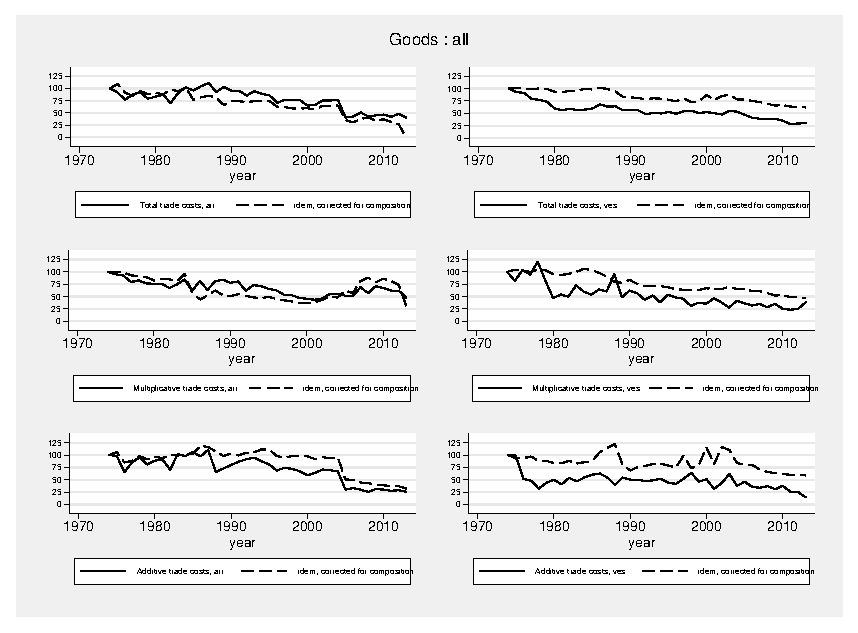
\includegraphics[height=8cm]
{graph_composition_all.pdf}
\end{center}
\end{figure}

As reported in Figures \ref{fig:totalTC_compeffects_excl_manuf} and \ref{fig:totalTC_compeffects_excl_primary}, both the ``pure'' transport costs and the unfitted measure, in the red dashed have regularly declined over the period in both sectors, by roughly the same order of magnitude (50\% in air, 60\% in vessel for overall transport costs, panels (c) and (f)). However the role of trade composition effects in accounting for this trend pattern differs depending on the sector.\\
In the manufacturing sector, Figure \ref{fig:totalTC_compeffects_excl_manuf}) reports a very similar time trend decomposition than what is obtained on the whole range of goods (Figure \ref{fig:totalTC_compeffects_excl}).  In air transport, most of the decrease can be imputed to the reduction of``ceteris paribus'' transport costs (the blue continuous line), trade composition effects playing virtually no role (Figure \ref{fig:totalTC_compeffects_excl_manuf}, left-hand panels (a), (b) and (c)). Trade composition effects matter more in vessel transport (Figure \ref{fig:totalTC_compeffects_excl_manuf}, right-hand panels (d), (e) and (f)), primarily in the ad-valorem component. As for the whole range of flows, the 60\% decrease in the unfitted transport costs in vessel can de decomposed in a 50\% decrease in the ``ceteris paribus'' transport costs (fitted), the 10\% remaining to trade composition effects.

The situation is strikingly different for primary goods only. In this case, it is in air transport that composition effects do matter (Figure \ref{fig:totalTC_compeffects_excl_primary}, left-hand panels (a), (b) and (c)), while we observe not much role for them in vessel transport (Figure \ref{fig:totalTC_compeffects_excl_primary}, left-hand panels (d), (e) and (f)). Furthermore, in air transport, composition effects matter by partially offsetting the decrease in the ``ceteris paribus'' transport costs (ie, implying a reduction in the ``raw'' transport costs over time much less pronounced than the fitted transport cost measures).

One explanation for the similarity between the results for the manufacturing goods trade and for total trade can be found in the share of primary goods in total flows as reported in Figure \ref{fig:Share_prim_goods}. In air transport, the share of primary goods in the total value of US imports is very small, around 10\%. Primary goods make a higher proportion of trade flows in vessel transport, especially over 1974-1982 (between 40\% and 60\%). On the following sub-period though, their share has fallen to 20-30\%. Given the modest proportion of primary goods in total import flows of the US economy compared to the manufactured sector, it is hence not surprising that the diagnosis made about the time trend of transport costs when all types of flows are considered is driven by the trend patterns that occur within the manufacturing sector.

\begin{figure}[htbp]
\caption{Share of primary goods in the value of total US imports}
\label{fig:Share_prim_goods}
\begin{center}
\includegraphics[height=6cm]
{Share_of_primary.pdf}
\end{center}
\end{figure}



\end{document}
